%************************************************
\chapter{Experimental setup}
\label{ch:detector}
%************************************************

\section{Introduction}
\label{sec:detector_introduction}

The experimental data were collected from the ATLAS particle detector at the Large Hadron Collider (LHC).
The following section will introduce LHC and the ATLAS particle detector.

\section{The Large Hadron Collider}
\label{sec:detector_LHC}

The Large Hadron Collider (LHC) was built in the border between France and Switzerland by the European Organization for Nuclear Research (CERN).
It is a circular particle collider underground with circumference 27 km.
Two beams of protons are accelerated in opposite directions, to almost the speed of light, and then collide with each other at the collision point.
The energy of each beam is 6.5 TeV, and hence the center-of-mass energy of the two beams $\sqrt{s}$ is 13 TeV, which is the energy used in this experiment.
At such a high energy, new physics phenomena are expected, including SUSY.
By analyzing the collision events, we can have a deeper understanding of the laws of nature.
Figure \ref{fig:detector_LHC_accelerator_complex} shows the schematic diagram of the CERN accelerator complex, which contains a series of accelerators, from low energy to high energy.
The dark blue big circle in figure \ref{fig:detector_LHC_accelerator_complex} represents the LHC, on which there are 4 particle detectors at 4 different interaction points (yellow points): ATLAS, CMS, LHCb and ALICE.

\begin{figure}
\centering
\includegraphics[width=\textwidth]{data/photo/detector/accelerator_complex.png}
\caption{The schematic diagram of the CERN accelerator complex, which shows a series of accelerators and facilities \cite{complex}.}
\label{fig:detector_LHC_accelerator_complex}
\end{figure}

Before the beam is injected into LHC, the protons are accelerated by a series of accelerators.
The journey of the protons starts from a tank of hydrogen gas.
The proton and the electron are separated by an electric field.
The protons are then accelerated to 50 MeV by Linac2, which is a linear accelerator.
The beam is then injected to the second accelerator called the Proton Synchrotron Booster (PSB), which accelerates the beam to 1.4 GeV.
After then, the beam is injected to the third accelerator called the Proton Synchrotron (PS), which pushes the beam to 25 GeV.
The fourth accelerator, called the Super Proton Synchrotron (SPS), further pushes the beam to 450 GeV.
Finally, the beam is injected to the two beam pipes of the LHC.
One of the beam moves in clockwise direction, while another beam moves in anti-clockwise direction.
Two beams collide at the collision point inside the ATLAS detector \cite{accelerator}.

The circular path of the proton beam is maintained by many superconducting electromagnets along the LHC tunnel.
There are 1232 main magnetic dipoles, and each of them generates a large magnetic field of 8.3 T.
In order to generate such a high magnetic field, the coils need to have very high current of 11,080 A, therefore superconducting coil need to be used to reduce the heat loss due to the electrical resistance.
The material of superconducting coil is niobium-titanium (NbTi).
To reach the condition for superconductivity, the electromagnets operate at a very low temperature, i.e. 1.9 K.
There are also 392 magnetic quadrupoles to squeeze the proton beam, so that the chance of proton-proton collision will be higher \cite{supermagnet,cryogenics}.

The protons in the beam are grouped into different bunches and there are about $10^{11}$ protons in each bunch.
The time-spacing between two adjacent bunches is 25 ns (or 50 ns in the previous experimental setup).
This means that two bunches collide at the collision point in each 25 ns.
For each bunch crossing, there are about 10 to 50 proton-proton interactions.
Hence, about $10^9$ proton-proton collisions are produced per second.

The interacting rate for a physics process $\frac{dN}{dt}$ is the product of the cross section of that physics process $\sigma$ and the instantaneous luminosity $\mathcal{L}$.
\begin{equation}
\frac{dN}{dt} = \sigma \mathcal{L}
\end{equation}
The instantaneous luminosity $\mathcal{L}$ is a measure of the interacting rate of two protons at the collision point, which depends on the particle beam parameters.
The instantaneous luminosity in this experiment is about $10^{34}$ cm$^{-2}$ s$^{-1}$ (or 10 nb$^{-1}$ s$^{-1}$).

\section{ATLAS detector}
\label{sec:detector_ATLAS}

A Toroidal LHC ApparatuS (ATLAS) is the particle detector used in this experiment \cite{ATLAS_doc}.
Figure \ref{fig:detector_ATLAS} shows the main components of the ATLAS detector.
\begin{figure}
\centering
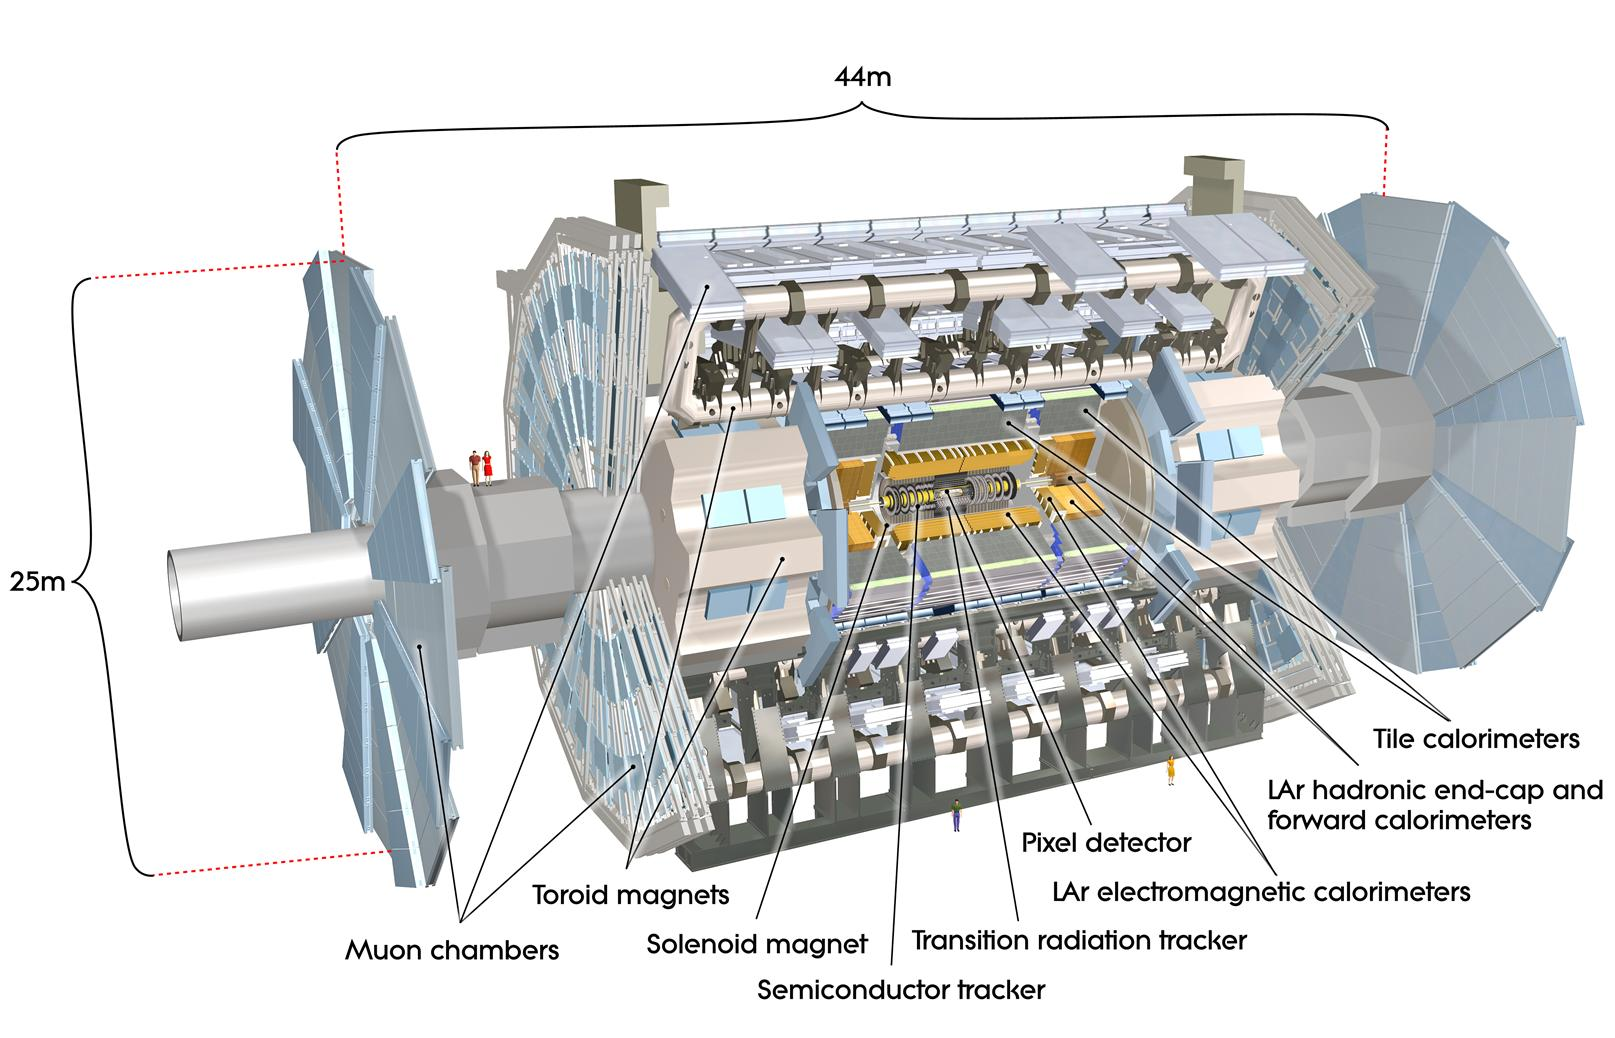
\includegraphics[width=\textwidth]{data/photo/detector/ATLAS.jpg}
\caption{The cut-away view of the ATLAS detector. It is 25 m high and 44 m long \cite{ATLAS_photo}.}
\label{fig:detector_ATLAS}
\end{figure}
Its height is 25 m, its length is 44 m and its weight is 7000 tonnes.
The ATLAS detector is a general purpose particle detector, which is consisted of 3 main components: the inner detector, the calorimeter and the muon spectrometer.
The heavy and hence short-lived particles will immediately decay into lighter particles.
The lighter particles and stable particles pass through different parts of the detectors.
These detectors measure the momentum and energy of the particles.
Figure \ref{fig:ATLAS_particles} shows how the ATLAS distinguishes different types of particle by using different components of the detector.
\begin{figure}
\centering
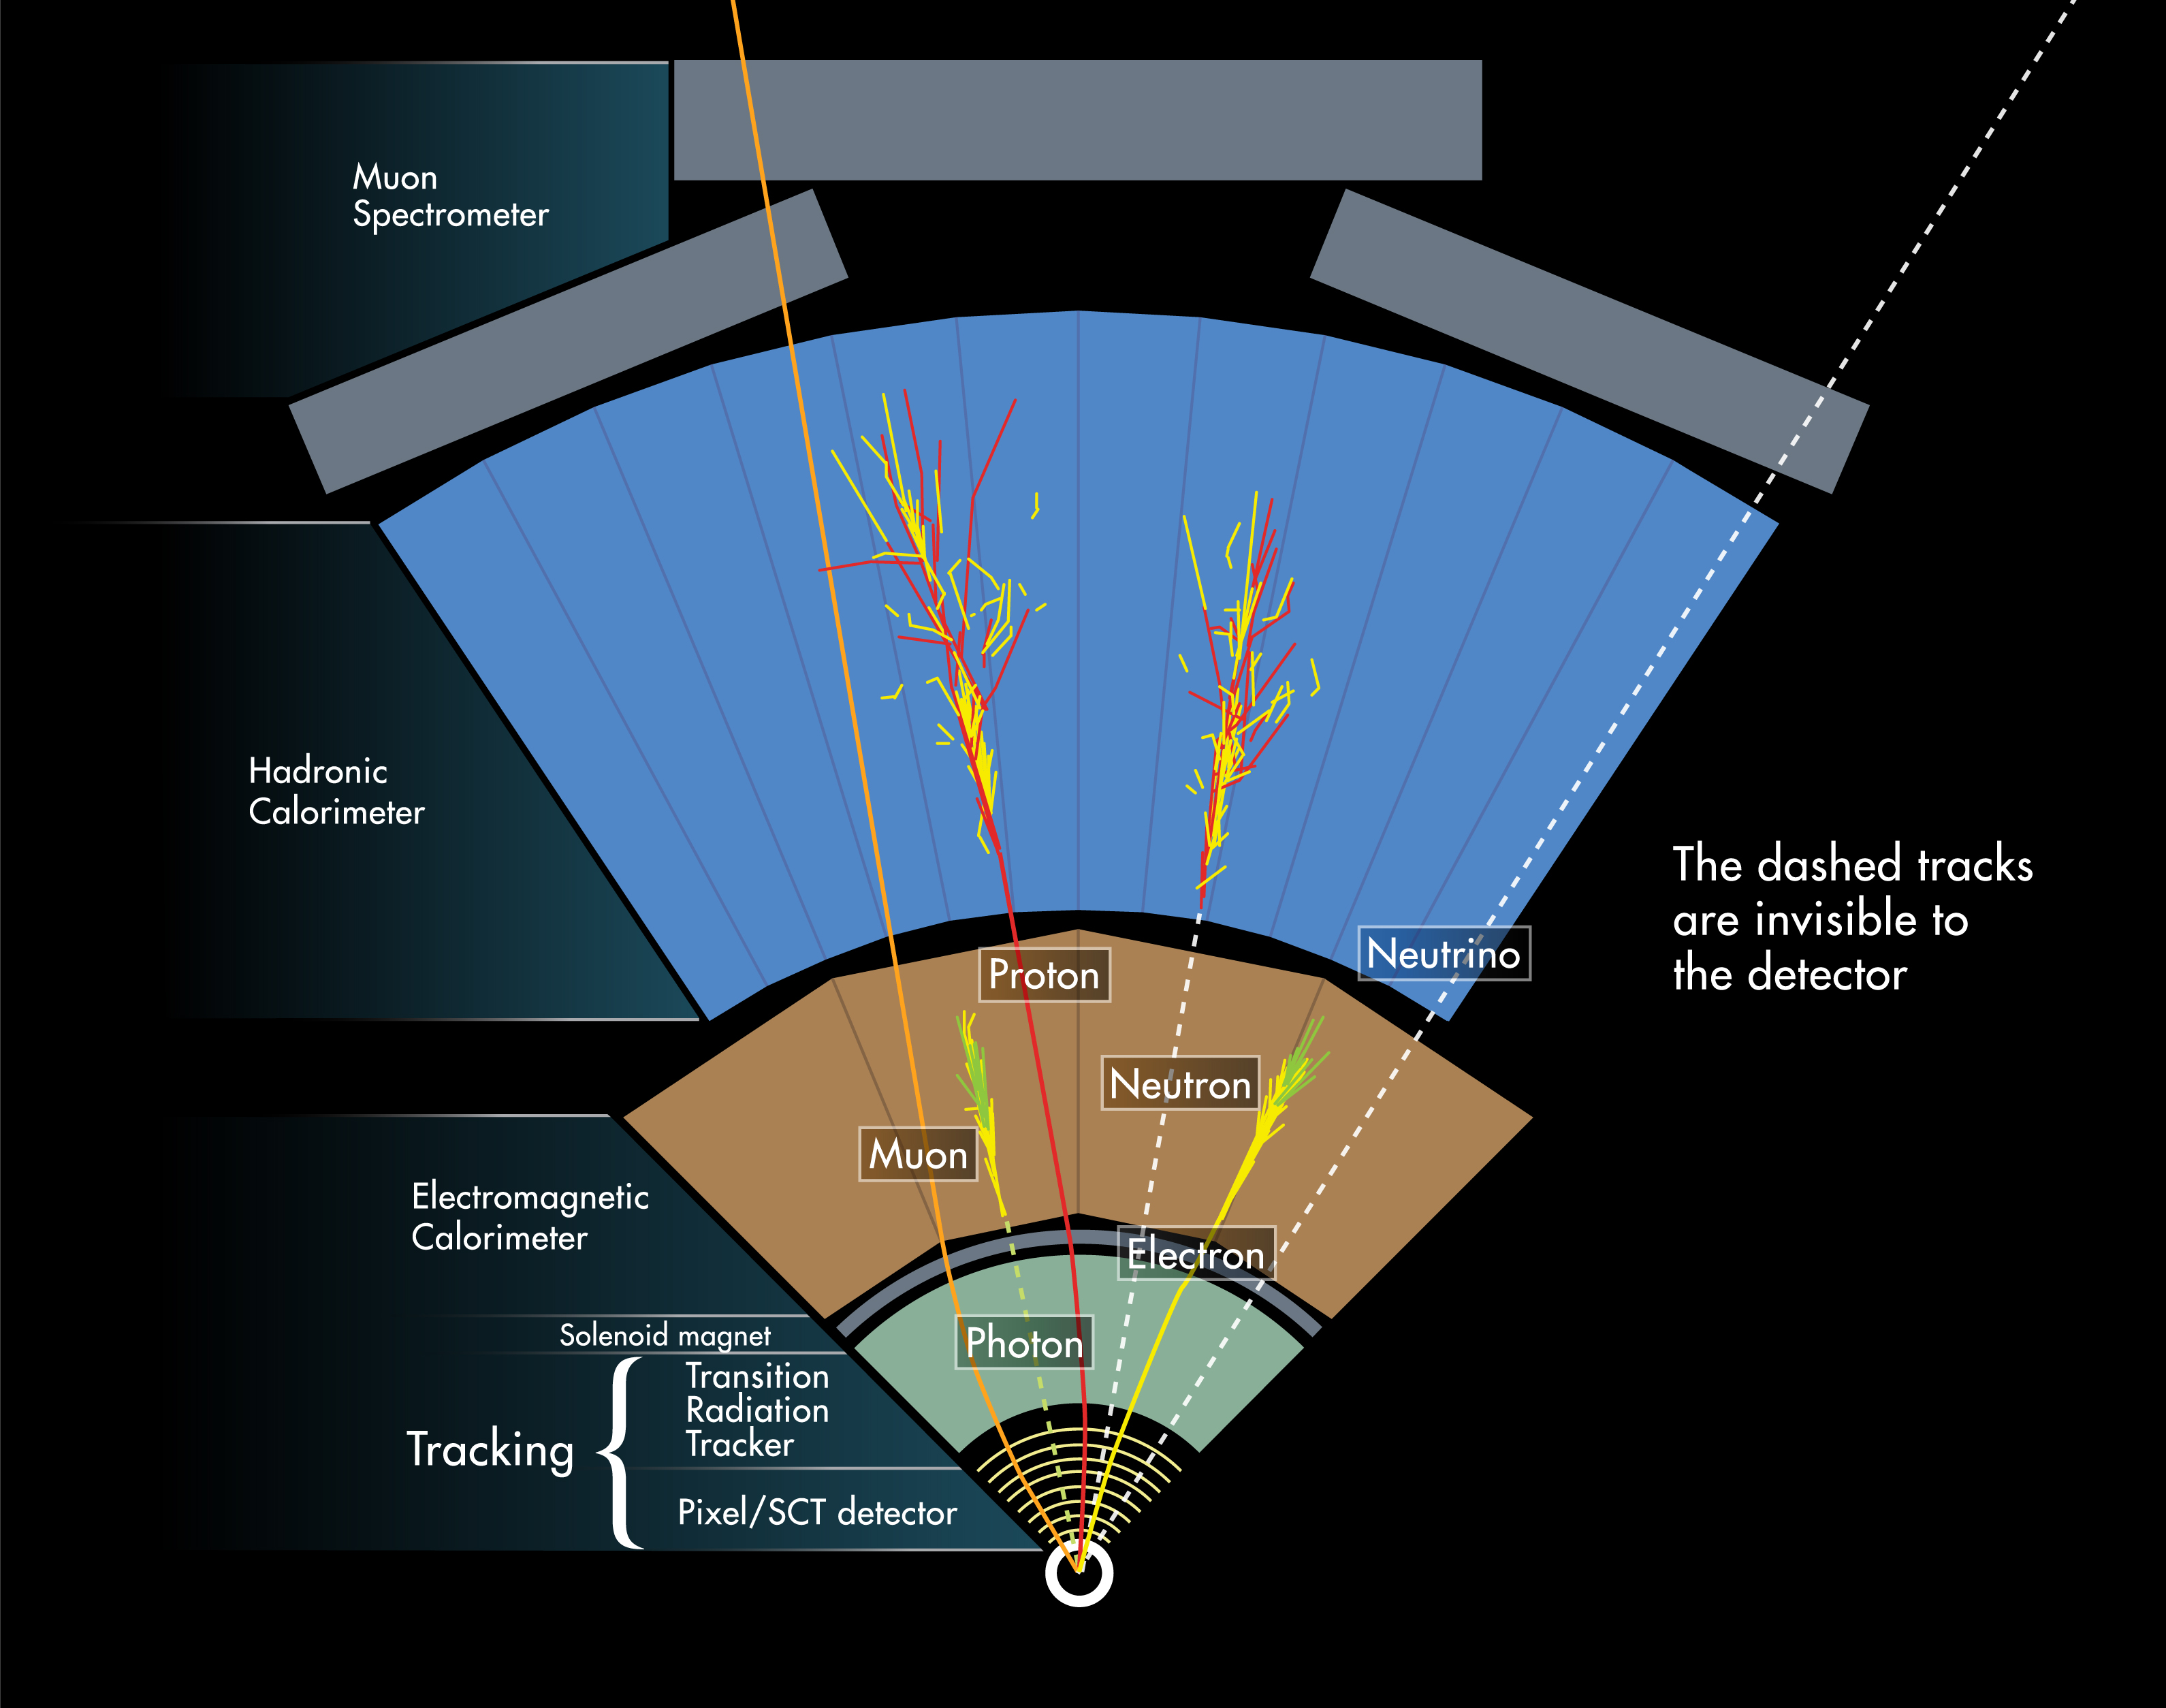
\includegraphics[width=\textwidth]{data/photo/detector/ATLAS_particles.jpg}
\caption{The cross section of the ATLAS detector. This shows different components of the ALTAS and how ATLAS detects different types of particles \cite{ATLAS_particles}.}
\label{fig:ATLAS_particles}
\end{figure}
The inner detector is surrounded by the solenoid, providing a strong magnetic field.
The magnetic field bends the charged particles and the inner detector can detect the paths of the charged particles and measure its momentum.
Photons and electrons deposit most of their energy in the electromagnetic calorimeter.
Hadrons(including protons and neutrons) and mesons deposit energy in the hadronic calorimeter.
Only muons and the neutrinos can reach the outermost muon spectrometer, but only muons can be detected by the muon spectrometer.
Neutrinos escape the ATLAS detector, which leads to missing energy.
In this design, different particles can be identified due to their own signature in different parts of ATLAS.

\begin{itemize}
\item \textbf{Electron} The track of an electron is measured by the inner detector and its energy deposits in the electromagnetic calorimeter.
\item \textbf{Proton} The tracks of protons are measured by the inner detector and their energies deposit in the hadronic calorimeter.
\item \textbf{Photon} No track is inside inner detector but its energy deposits in the electromagnetic calorimeter.
\item \textbf{Neutron} No track is inside inner detector but its energy deposits in the hadronic calorimeter.
\item \textbf{Muon} The tracks of muons are measured by the inner detector and the muon spectrometer. They nearly do not deposit their energies into the calorimeter and escape the detector.
\item \textbf{Neutrino} Neutrinos cannot be detected, which contributes to the missing momentum.
\end{itemize}

\subsection{The coordinate system and basic variables}
The nominal collision point is defined as the origin of the coordinate system.
The z-axis is along the anticlockwise beam direction.
The positive x-axis is pointing to the centre of the LHC ring.
The positive y-axis is in the upward direction.
The ATLAS detector is symmetric about the x-y plane.

The impact parameters of the track of a particle are $z_0$ and $d_0$, described in figure \ref{fig:impact_parameter}.
The nearest point of the track to the z-axis is marked by the small circle in the figure, with the smallest distance $d_0$.
The z-coordinate of the nearest point is $z_0$.

\begin{figure}
\centering
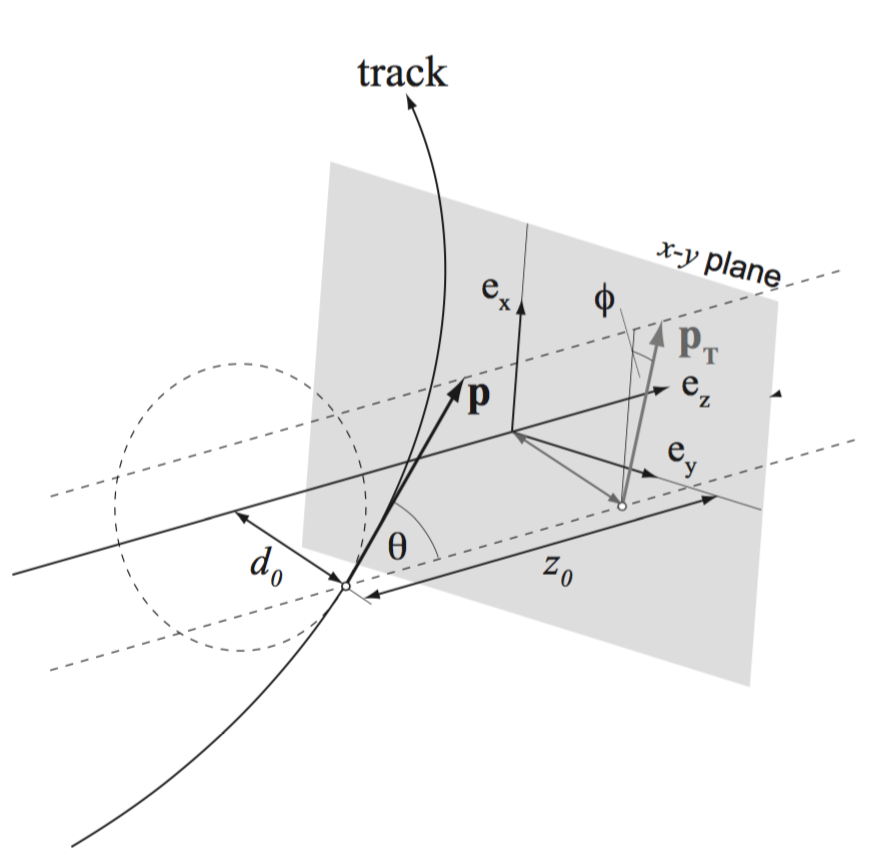
\includegraphics[width=0.6\textwidth]{data/photo/detector/impact_parameter.png}
\caption{This figure shows how the impact parameters $z_0$ and $d_0$ are defined by the nearest point (the small circle) of the track to the z-axis. It also shows how the azimuthal angle $\phi$ and the polar angle $\theta$ of the momentum $\bf{p}$ are defined. $p_T$ is the projection of the momentum $\bf{p}$ onto the x-y plane.}
\label{fig:impact_parameter}
\end{figure}

The figure also shows the momentum $\bf{p}$ of the particle when it passes through the nearest point.
The azimuthal angle $\phi$ and the polar angle $\theta$ of the momentum $\bf{p}$ are defined as usual in the spherical coordinate system.
The polar angle $\theta$ is the angle between the momentum $\bf{p}$ and the positive z-direction.
The pseudorapidity $\eta$ is defined as:
\begin{equation}
\eta = - \ln \Big( \tan \frac{\theta}{2} \Big)
\end{equation}
Different polar angles $\theta$ corresponding to different values of pseudorapidity $\eta$ are shown in figure \ref{fig:pseudorapidity}.
The positive values of pseudorapidity $\eta$ correspond to $0 <\theta< \frac{\pi}{2}$, while the negative values of pseudorapidity $\eta$ correspond to $\frac{\pi}{2} <\theta< \pi$.
The values of pseudorapidity $\eta$ are reflective symmetric about the x-y plane.
\begin{align}
( \eta \text{ at } \theta = \pi - x) &= - \ln \Big( \tan \frac{\pi - x}{2} \Big) \\
&= - \ln \Big( \tan (\frac{\pi}{2} - \frac{x}{2}) \Big) \\
&= - \ln \Big( \frac{1}{ \tan \frac{x}{2} } \Big) \\
&= - \Big( - \ln \Big( \tan \frac{x}{2} \Big) \Big) \\
&= - ( \eta \text{ at } \theta = x)
\end{align}
The ATLAS detector covers the region where $|\eta| < 4.9$, but the reconstructed objects are often restricted to $|\eta| < 2.5$.

\begin{figure}
\centering
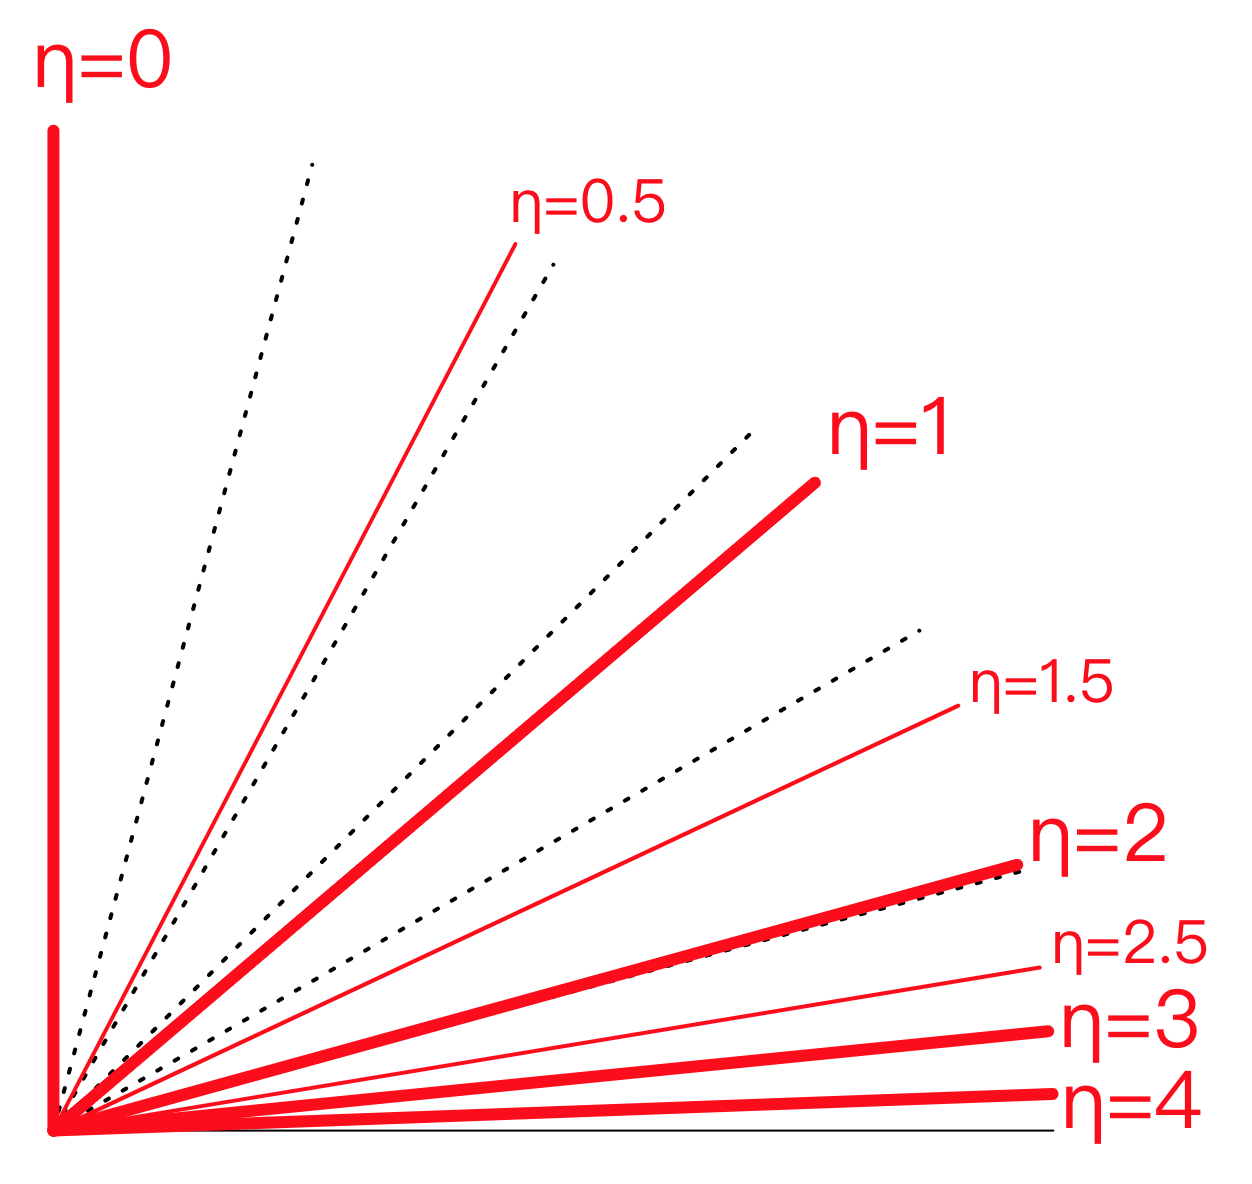
\includegraphics[width=0.6\textwidth]{data/photo/detector/pseudorapidity.png}
\caption{The red lines show different directions corresponding to different positive values of pseudorapidity \cite{pseudorapidity}.}
\label{fig:pseudorapidity}
\end{figure}

The projection of the nearest point onto the x-y plane is also shown in figure \ref{fig:impact_parameter}.
The transverse momentum of a particle, denoted by $\bf{p}_T$, is the projection of its momentum $\bf{p}$ onto the x-y plane, as shown in the figure.
The azimuthal angle $\phi$ of the momentum $\bf{p}$ is the azimuthal angle of $\bf{p}_T$ in the two-dimensional polar coordinate system on the x-y plane.
The magnitude of $\bf{p}_T$ is denoted by $p_T$.
\begin{equation}
p_T = \sqrt{p_x^2 + p_y^2}
\end{equation}
In the following chapter, the term ``transverse momentum" $p_T$ refer to the magnitude of $\bf{p}_T$.

The distance $\Delta R$ in the pseudorapidity-azimuthal angle space of two particles is defined as:
\begin{equation}
\Delta R = \sqrt{(\Delta \phi) ^2 + (\Delta \eta) ^2}
\end{equation}
It measures the angular separation of the momentum of two particles.

\subsection{The magnetic system}
\label{sec:magnetic_system}
There is a thin superconducting solenoid magnet around the inner detector, which generates a 2 T magnetic field in the z-direction inside the inner detector.
There are also 3 large superconducting toroids around the calorimeter: one for barrel and two for end-caps.
Each toroid consists of eight coils arranged symmetrically, which provide magnetic field in the $\phi$-direction for the muon spectrometer.
The end-cap toroids are rotated by 22.5$^{\circ}$ relative to the barrel toroid, in order to optimize the magnetic field at the region between the two coil systems.
The strength of the magnetic field is 0.5 T in the barrel region and 1 T in the end-cap region.
All these magnets are shown in figure \ref{fig:magnetic_system}.

\begin{figure}
\centering
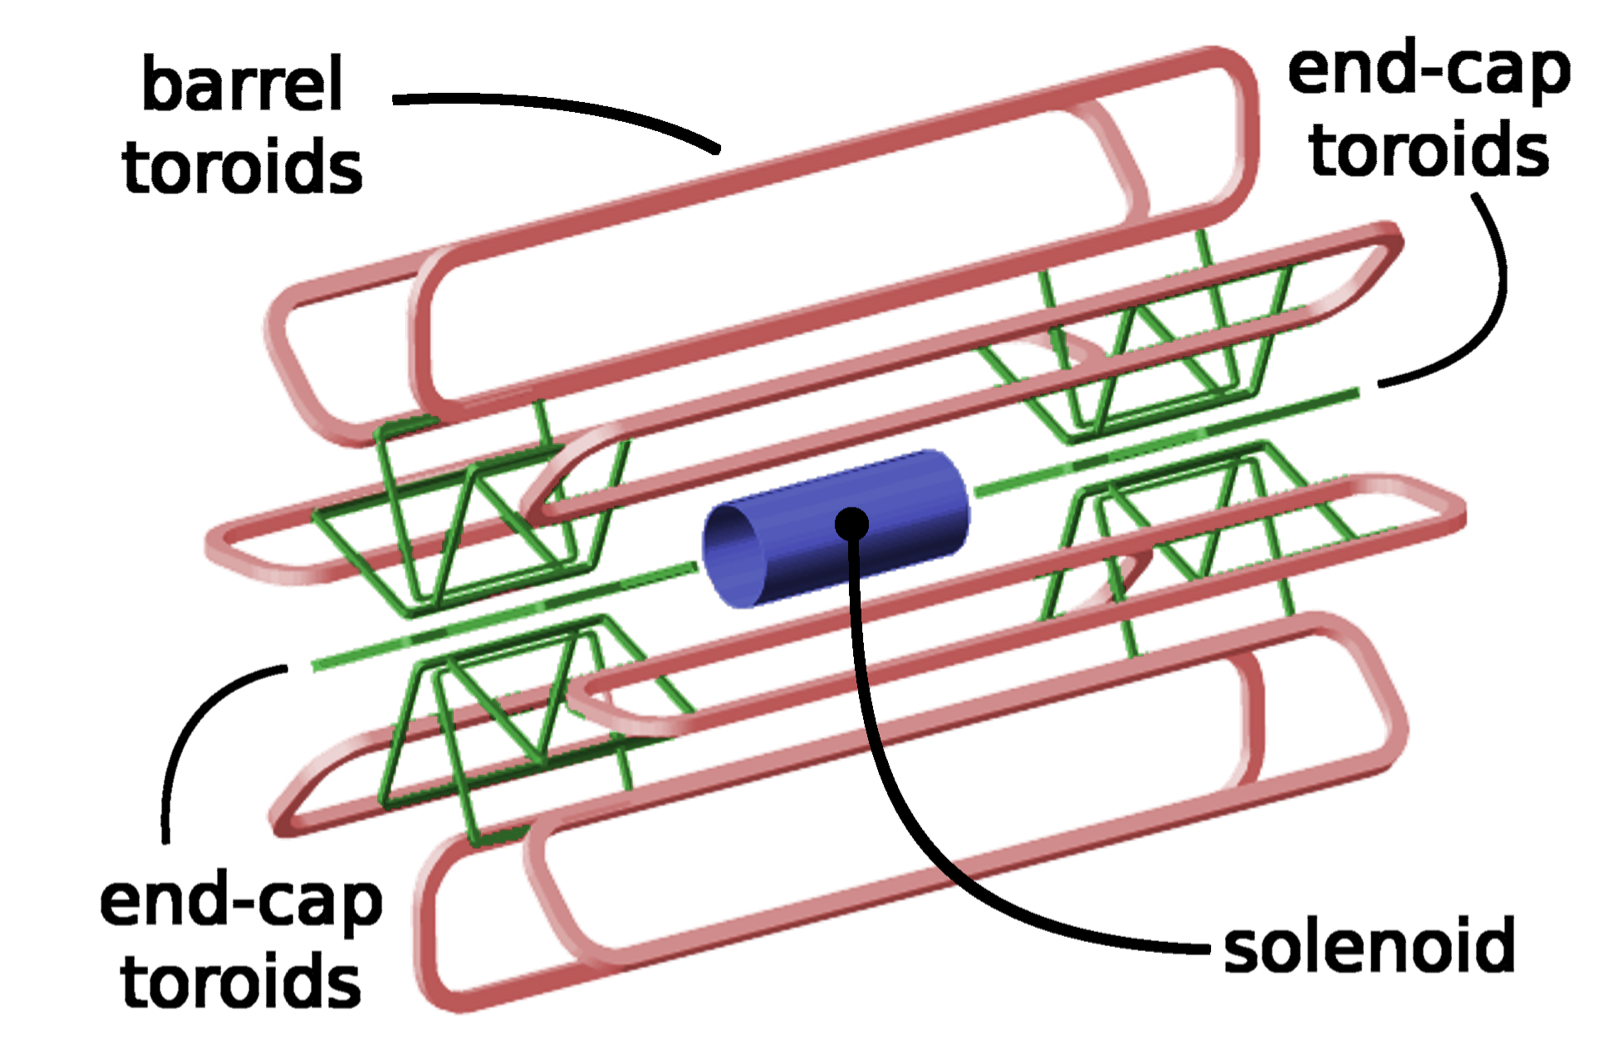
\includegraphics[width=0.6\textwidth]{data/photo/detector/magnet.png}
\caption{Schematic view of the magnetic system of the ATLAS detector \cite{magnetic_system}.}
\label{fig:magnetic_system}
\end{figure}

\subsection{The inner detector}
The inner detector is a particle tracker.
For each collision, thousands of particles will be produced within $|\eta| < 2.5$.
It measures the tracks of charged particles, the momentum of the charged particles and the position of the vertices.
Figure \ref{fig:detector_inner_whole} shows the whole structure of the inner detector.
The inner detector consists of 3 sub-detectors from inner to outer: the pixel detector, the silicon microstrip tracker (SCT) and the transition radiation tracker (TRT).
Each part further divides into two parts: the barrel region with smaller $|\eta|$ and the end-cap region with larger $|\eta|$.
Figure \ref{fig:detector_inner_detail} shows the radius R of the 3 sub-detectors from the beam, and figure \ref{fig:detector_inner_size} shows the shapes and the orientations of each sensor and the $\eta$ coverage, in both the barrel and the end-cap regions.
The $\eta$ coverage for the inner detector is $|\eta| < 2.5$.
The shapes and the orientations of the sensors are different in the barrel and the end-cap regions.
In the barrel region, the shape and the orientation of the sensors is concentric cylinder shells around the beam axis, while in the end-cap region, they are disks perpendicular to the beam axis.
\begin{figure}
\centering
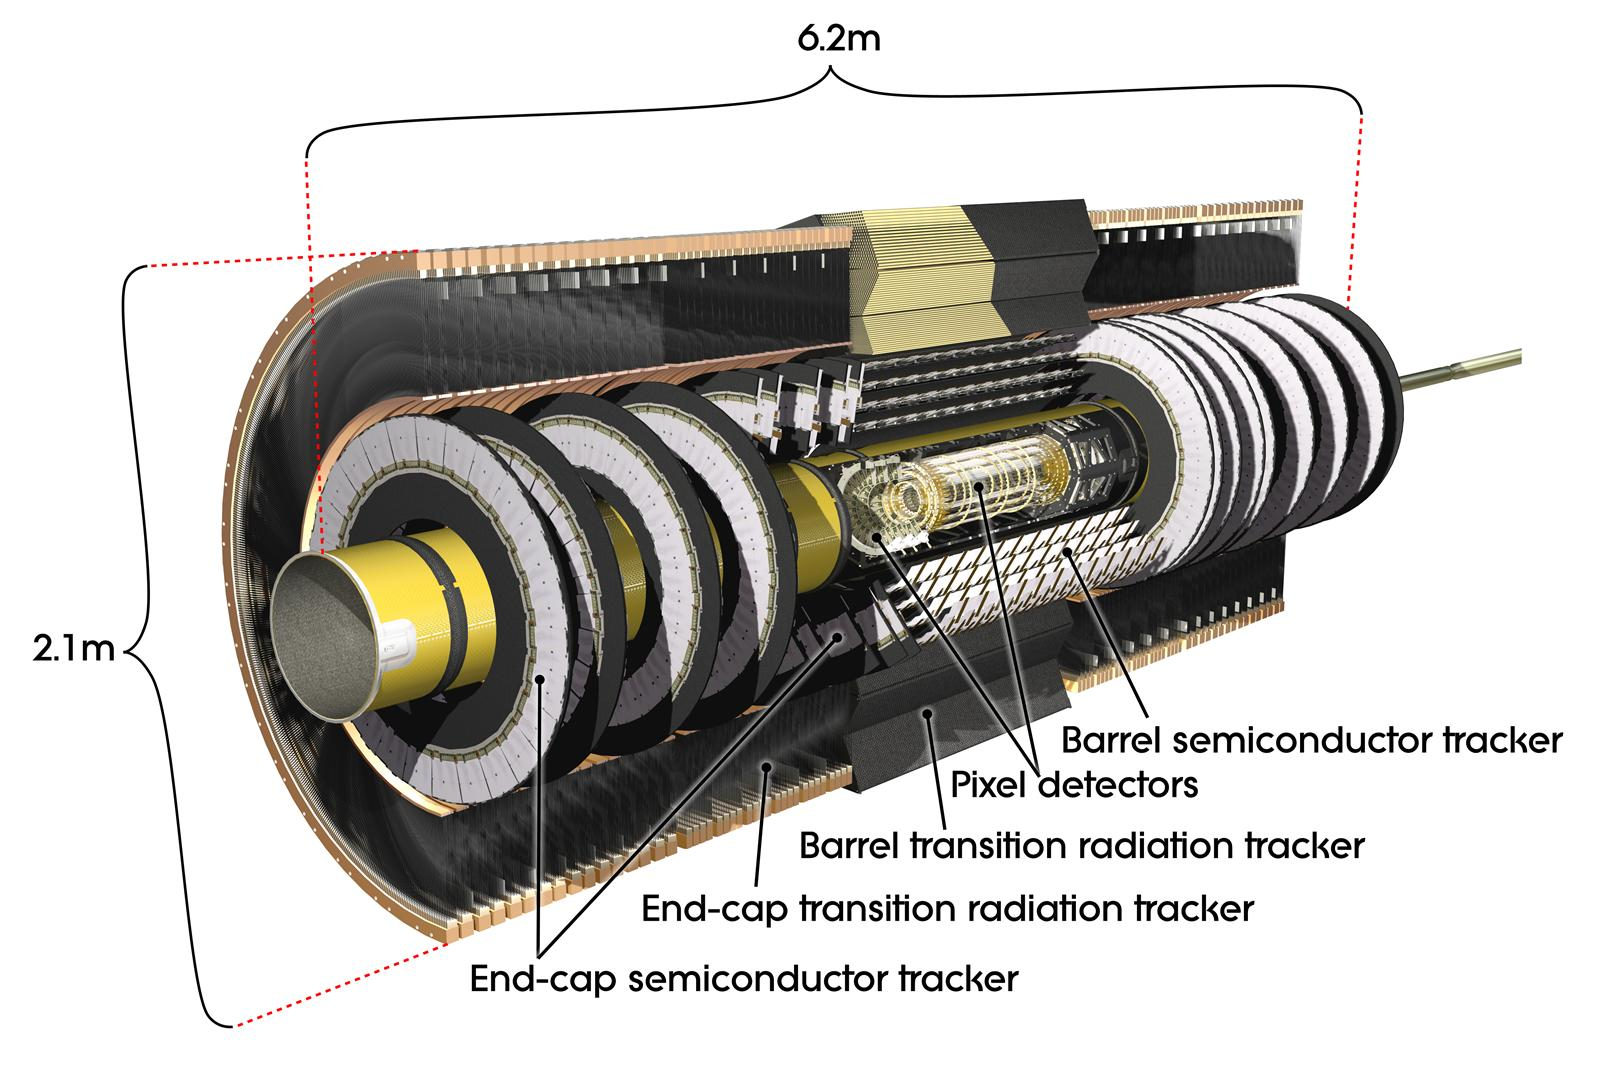
\includegraphics[width=\textwidth]{data/photo/detector/inner_whole.jpg}
\caption{The whole structure of the ATLAS inner detector \cite{inner_photo}.}
\label{fig:detector_inner_whole}
\end{figure}
\begin{figure}
\centering
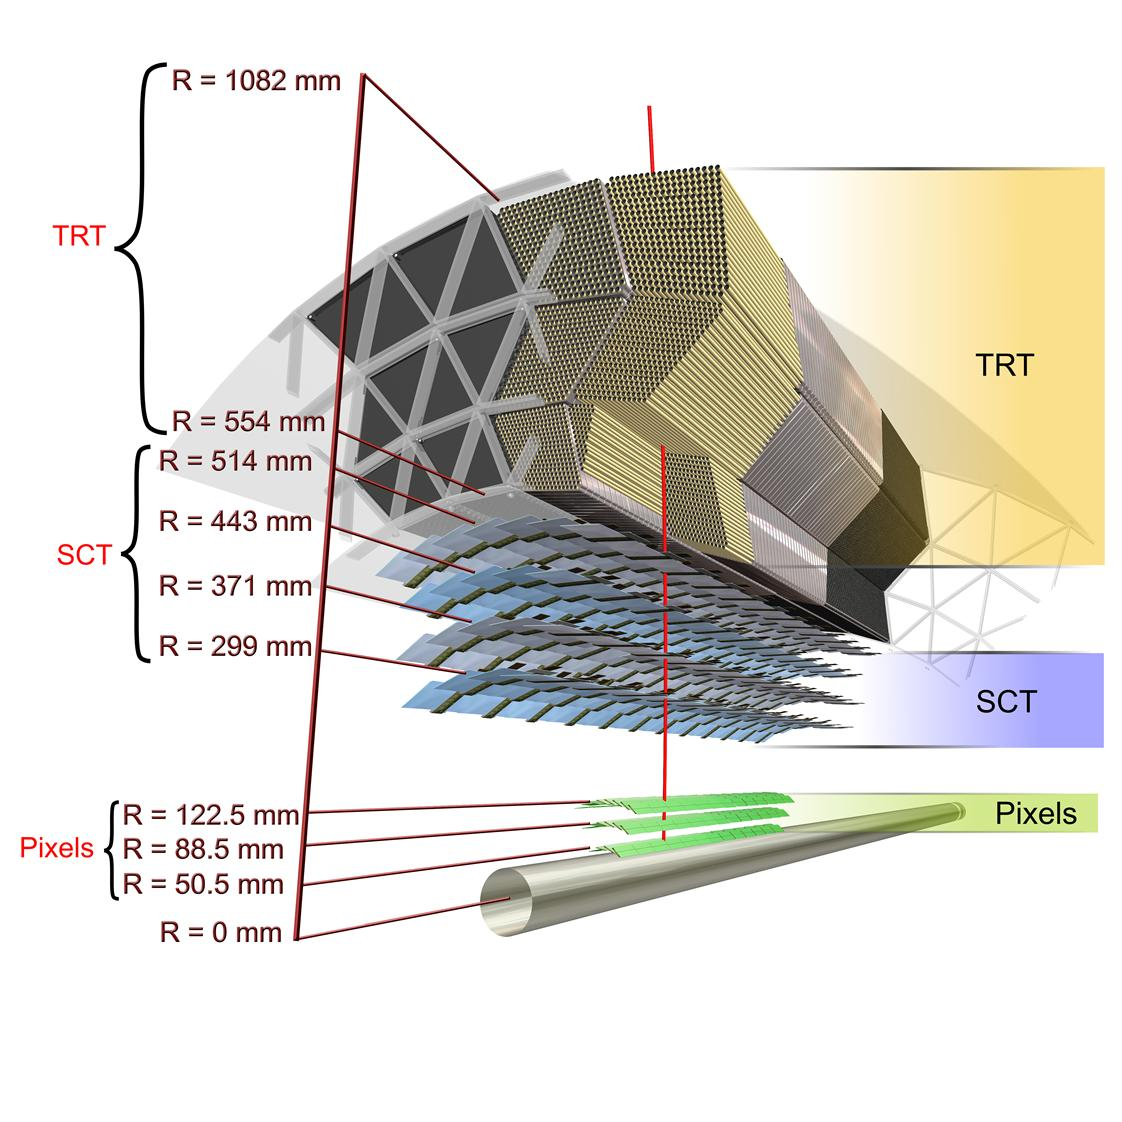
\includegraphics[width=\textwidth]{data/photo/detector/inner_detail.jpg}
\caption{The radius R from the beam for the 3 components: pixel, SCT and TRT \cite{inner_photo}.}
\label{fig:detector_inner_detail}
\end{figure}
\begin{figure}
\centering
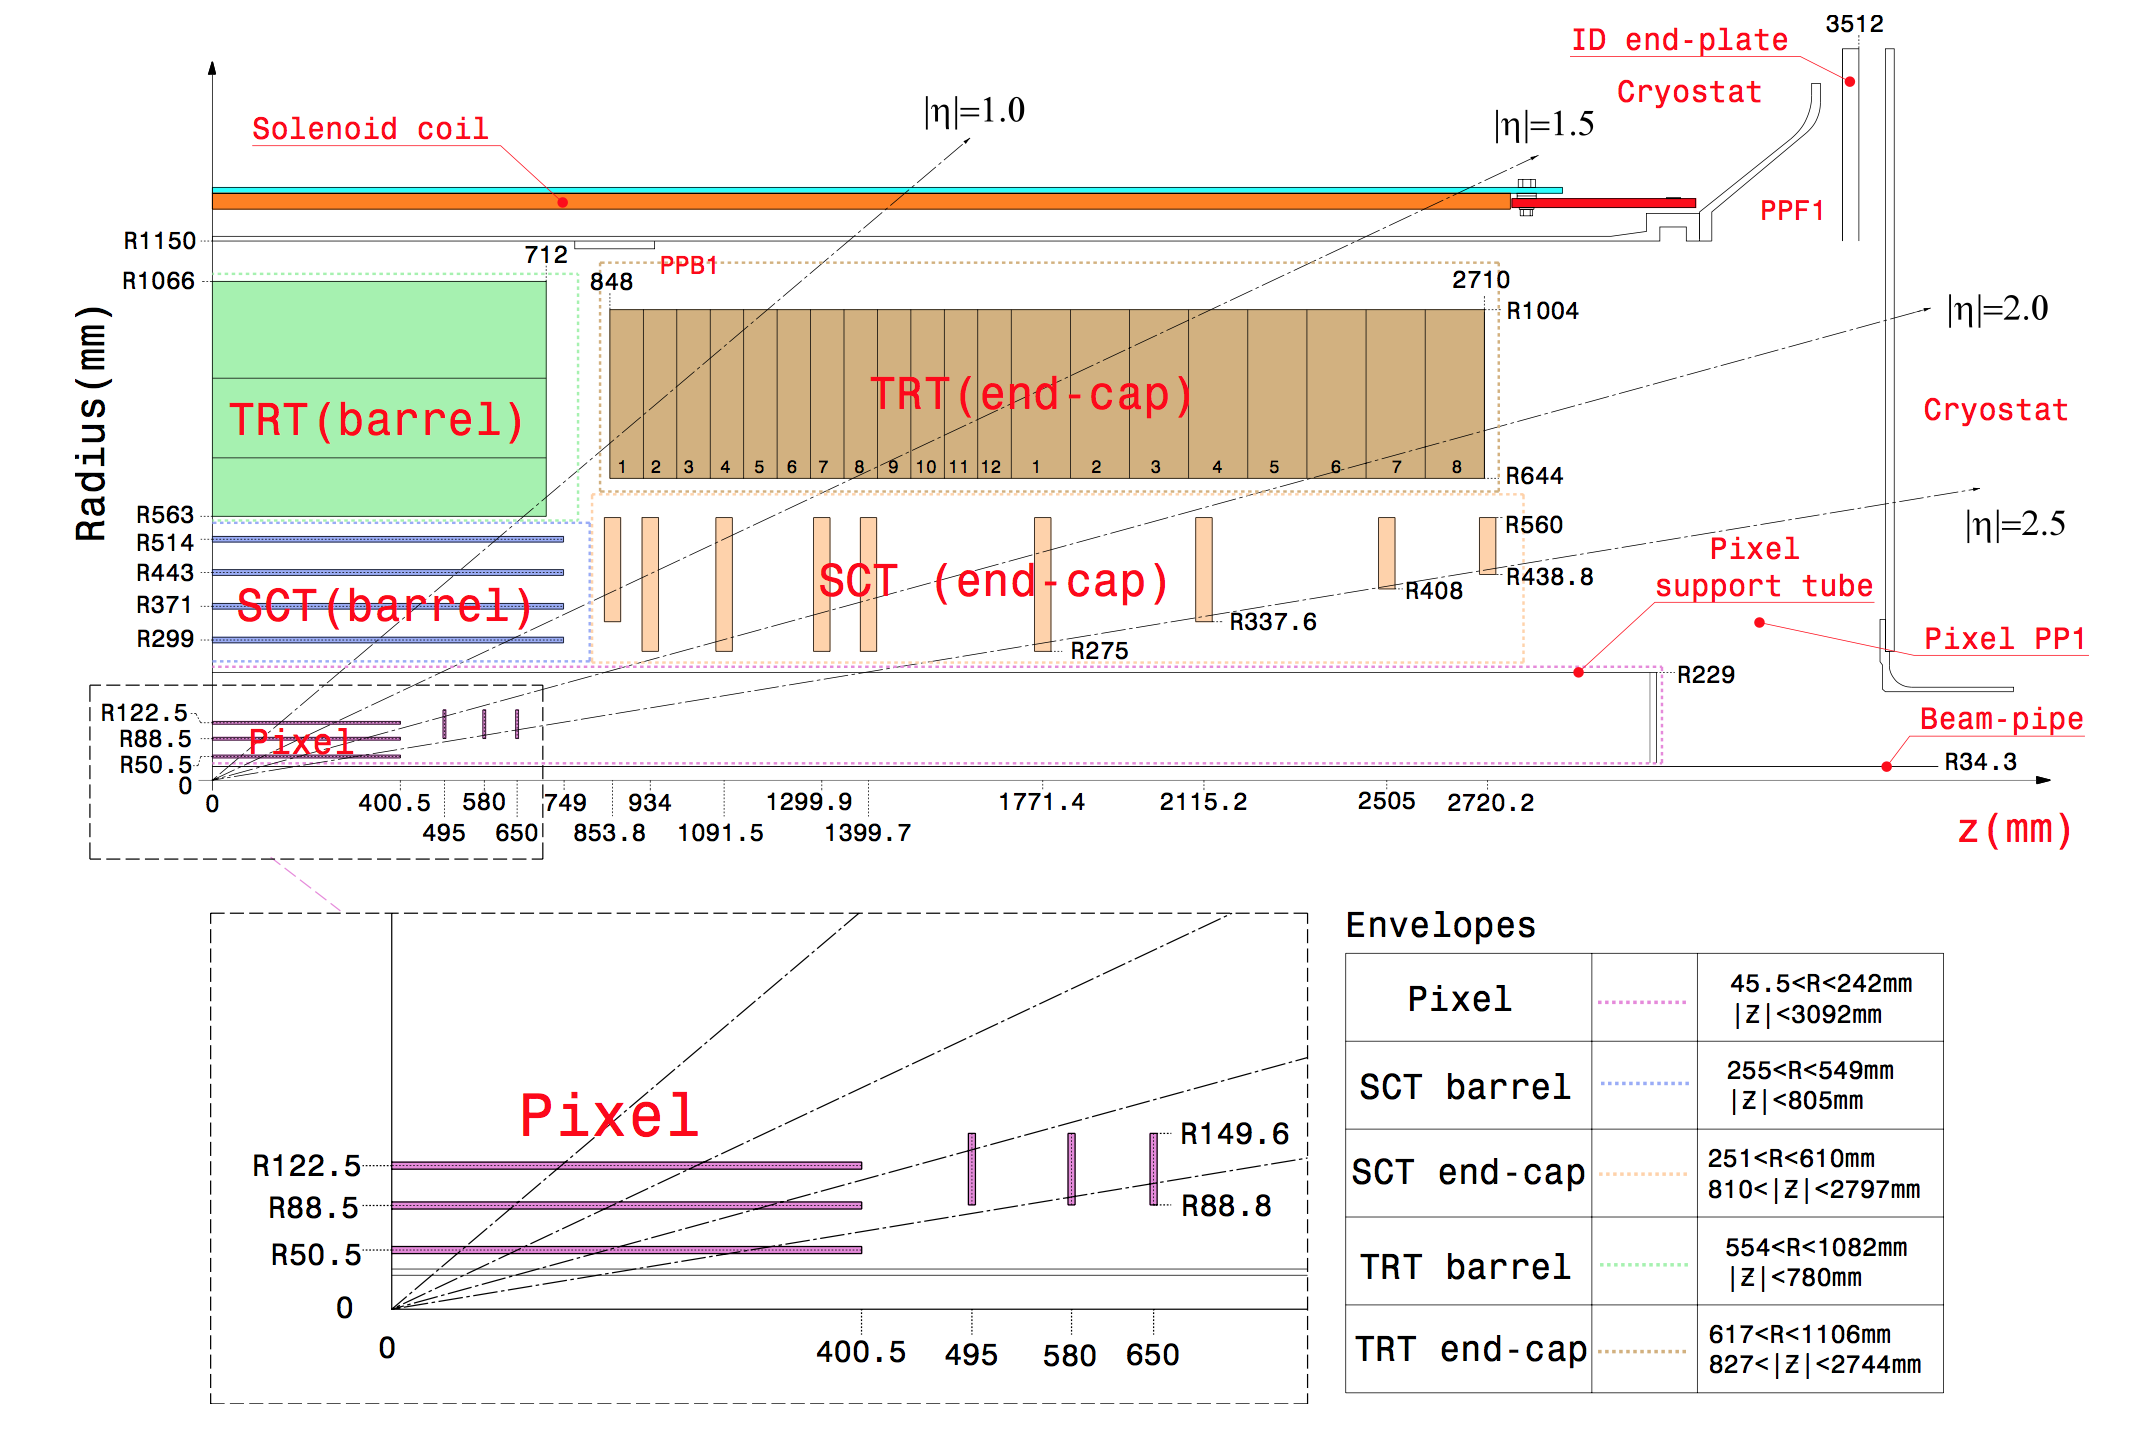
\includegraphics[width=\textwidth]{data/photo/detector/inner_size.png}
\caption{The shapes, the orientations and the $\eta$ coverage for each sensor \cite{ATLAS_doc}.}
\label{fig:detector_inner_size}
\end{figure}

The precision tracking detectors (pixels and SCT) has high resolution in space by using discrete space-points to detect the track of a charged particle, with the cutting-edge technology, in order to achieve the good performance of the inner detector.
When the particle moves inside the inner detector, there are averagely 36 hits per track.
By recording the positions of these hits, the path of the particle can be reconstructed.
The whole inner detector is immersed in a 2 T magnetic field generated by the solenoid magnet, therefore the path of any charged particles will be bent.
By measuring the curvature of the path, the charge and momentum of the particle are measured.
The equation for the circular path is
\begin{equation}
\frac{d\mathbf{p}}{dt} = q(\mathbf{v} \times \mathbf{B})
\end{equation}
where the relativistic momentum $\mathbf{p} = \gamma m \mathbf{v}$.
\begin{align}
\frac{d\mathbf{p}}{dt} &= q( \frac{\mathbf{p}}{\gamma m} \times \mathbf{B}) \\
&= \frac{q}{\gamma m} (\mathbf{p} \times \mathbf{B})
\end{align}
From this equation, we can get the angular frequency $\omega$,
\begin{align}
\omega &= \frac{qB}{\gamma m} \\
\frac{v}{r} &= \frac{qB}{\gamma m} \\
\frac{1}{r} &= \frac{qB}{\gamma m v} \\
\frac{1}{r} &= \frac{qB}{p} \\
p &= rqB
\end{align}
We can calculate the momentum of the particle from the curvature of track $1/r$, the charge and the magnetic field strength.

\subsubsection{Pixel detector}
The pixel detector is the innermost part of the inner detector, therefore it has to withstand the highest amount of radiation from the interaction point.
As shown in figure \ref{fig:detector_inner_size}, there are 3 layers of cylinder in the barrel region at radii 50.5 mm, 88.5 mm and 122.5 mm, and 3 layers of disk for each end-cap region at z = 495 mm, 580 mm and 650 mm.
There are in total 1744 modules in the pixel detectors.
Each module is identical, and has the size of 19mm$\times$63mm.
The module has 47232 pixels, with the size of 50$\mu$m$\times$400$\mu$m.
There are in total 80 million pixels for the whole pixel detector.
Each pixel measures the position with an accuracy of 10$\mu$m$\times$115$\mu$m.

The sensors in the module are made with planar n$^{+}$-in-n type of silicon with 250 $\mu$m thick, where n$^{+}$-type at the readout side (i.e. the electronics chip) and n-type at another side.
When charged particles pass through the silicon, electrons are produced and attracted to the anode, which is attached to an electronics chip with 180 $\mu$m thick.

The innermost layer of pixels at radius 50.5 mm is very important for measuring the secondary vertices of the long-lived b-hadrons.
It helps identify the b-jets (jets originating from bottom quarks), which are the decay products of the top quarks and Higgs bosons.

\subsubsection{SCT}
The SCT is in the middle part of the inner detector.
As shown in figure \ref{fig:detector_inner_size}, there are 4 layers of cylinder in the barrel region and 9 layers of disk for each end-cap region.
There are 4088 modules in the SCT and 6.3 million pixels.
Each module has the thickness of 300 $\mu$m.
It has a thermally conductive base-board in the middle, which provides the cooling of the sensor.
The p-in-n silicon sensors are glued on each side of the base-board.
The working principle is similar to the pixel detector.
Each sensor has the spatial resolution of 17$\mu$m$\times$580$\mu$m.

\subsubsection{TRT}
The TRT is the outermost part of the inner detector.
It detects the track of the charged particle, and help distinguishing the electrons from other charged hadrons.
It is a straw tube gaseous detector, with 96 TRT modules in the barrel and 20 TRT modules on each end-cap.
There are 52544 straws in the barrel and 122880 straws in the end-cap.
Each straw tube is a polyimide drift straw tube with 144 cm long and 4 mm diameter.
It is filled with a non-flammable gas mixture of 70\% Xe, 27\% CO$_2$ and 3\% O$_2$.
When a charged particle passes through the gas, it ionizes the gas and produces transition radiation.
The transition radiation further ionizes the gas and produces free electrons, which are attracted to the wire at the center of the straw tube.
The electrons can be identified by detecting the amount of transition radiation, because electrons emit more transition radiation than other charged hadrons, like pions.

The TRT has the spatial resolution of 130$\mu$m in the R-$\phi$ plane.
The spatial resolution of z is determined by the length of the straw tube, i.e. 144 cm.

\subsection{Calorimeter}
The calorimeter measures the energy of the particle.
Besides the measurement of the energy of the particles, it also helps identifying different particles like electrons, photons and jets.
It is because different particles have different signature when the particle deposits its energy to the calorimeters.
It contains two types of calorimeters: the electromagnetic calorimeter and the hadronic calorimeter.
The electromagnetic calorimeter is designed to measure the energy of electrons and photon, while the hadronic calorimeter is to measure the energy of the hadrons like protons, neutrons and mesons.
The figure \ref{fig:calorimeter_whole} shows the calorimeter system of the ATLAS detector.
In the barrel region, the Liquid Argon (LAr) electromagnetic calorimeter (ECal) works as an electromagnetic calorimeter, while the tile calorimeter (TileCal) works as a hadronic calorimeter.
In the end-cap region, the LAr ElectroMagnetic End-Cap (EMEC) calorimeter works as an electromagnetic calorimeter, while the LAr Hadronic End-Cap (HEC) calorimeter works as a hadronic calorimeter.
In the forward region, the LAr Forward Calorimeter (FCal) has three layers: one is electromagnetic and two are hadronic.
Figures \ref{fig:calorimeter_endcap1} and \ref{fig:calorimeter_endcap2} show the schematic view for one side of the end-cap and forward calorimeter.
The large coverage $|\eta| < 4.9$ is to ensure a good measurement of the missing energy ($E_T^{\text{miss}}$).

\begin{figure}
\centering
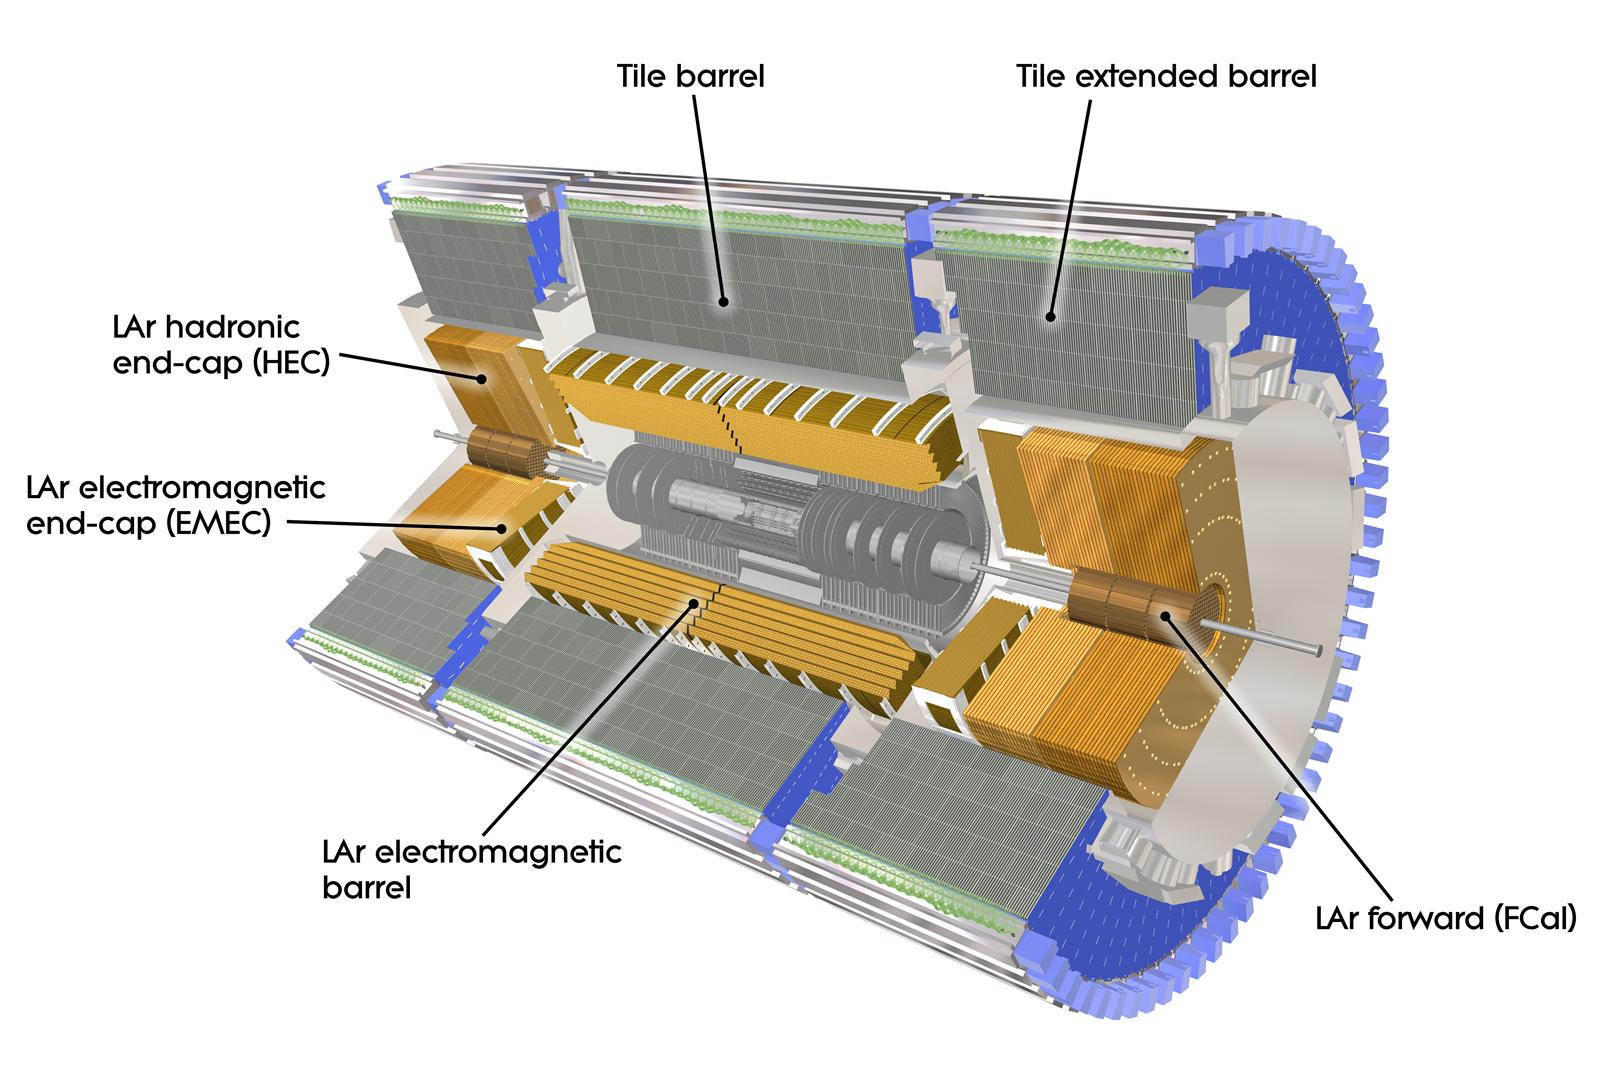
\includegraphics[width=\textwidth]{data/photo/detector/calorimeter_whole.jpg}
\caption{Schematic view for the calorimeter system of the ATLAS detector \cite{calorimeter_whole}.}
\label{fig:calorimeter_whole}
\end{figure}

\begin{figure}
\centering
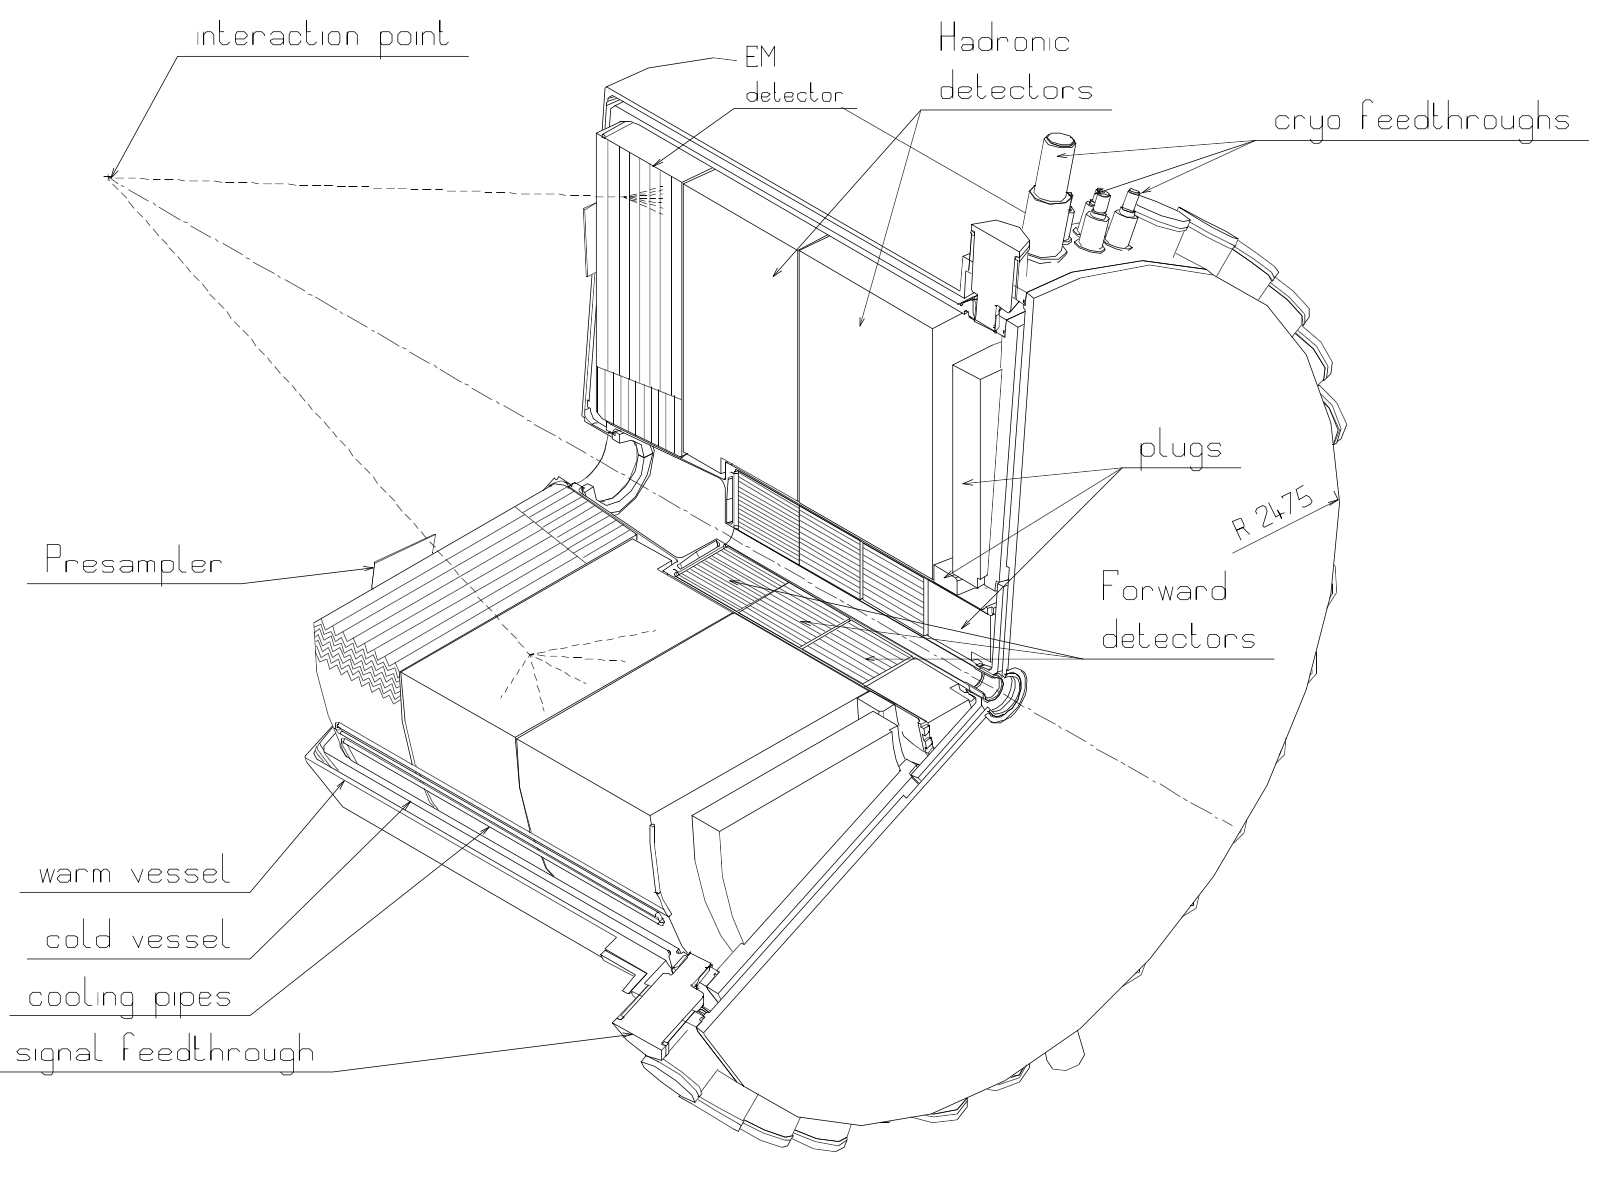
\includegraphics[width=\textwidth]{data/photo/detector/endcap1.png}
\caption{Schematic view for one side of the end-cap and forward calorimeter \cite{calorimeter}.}
\label{fig:calorimeter_endcap1}
\end{figure}

\begin{figure}
\centering
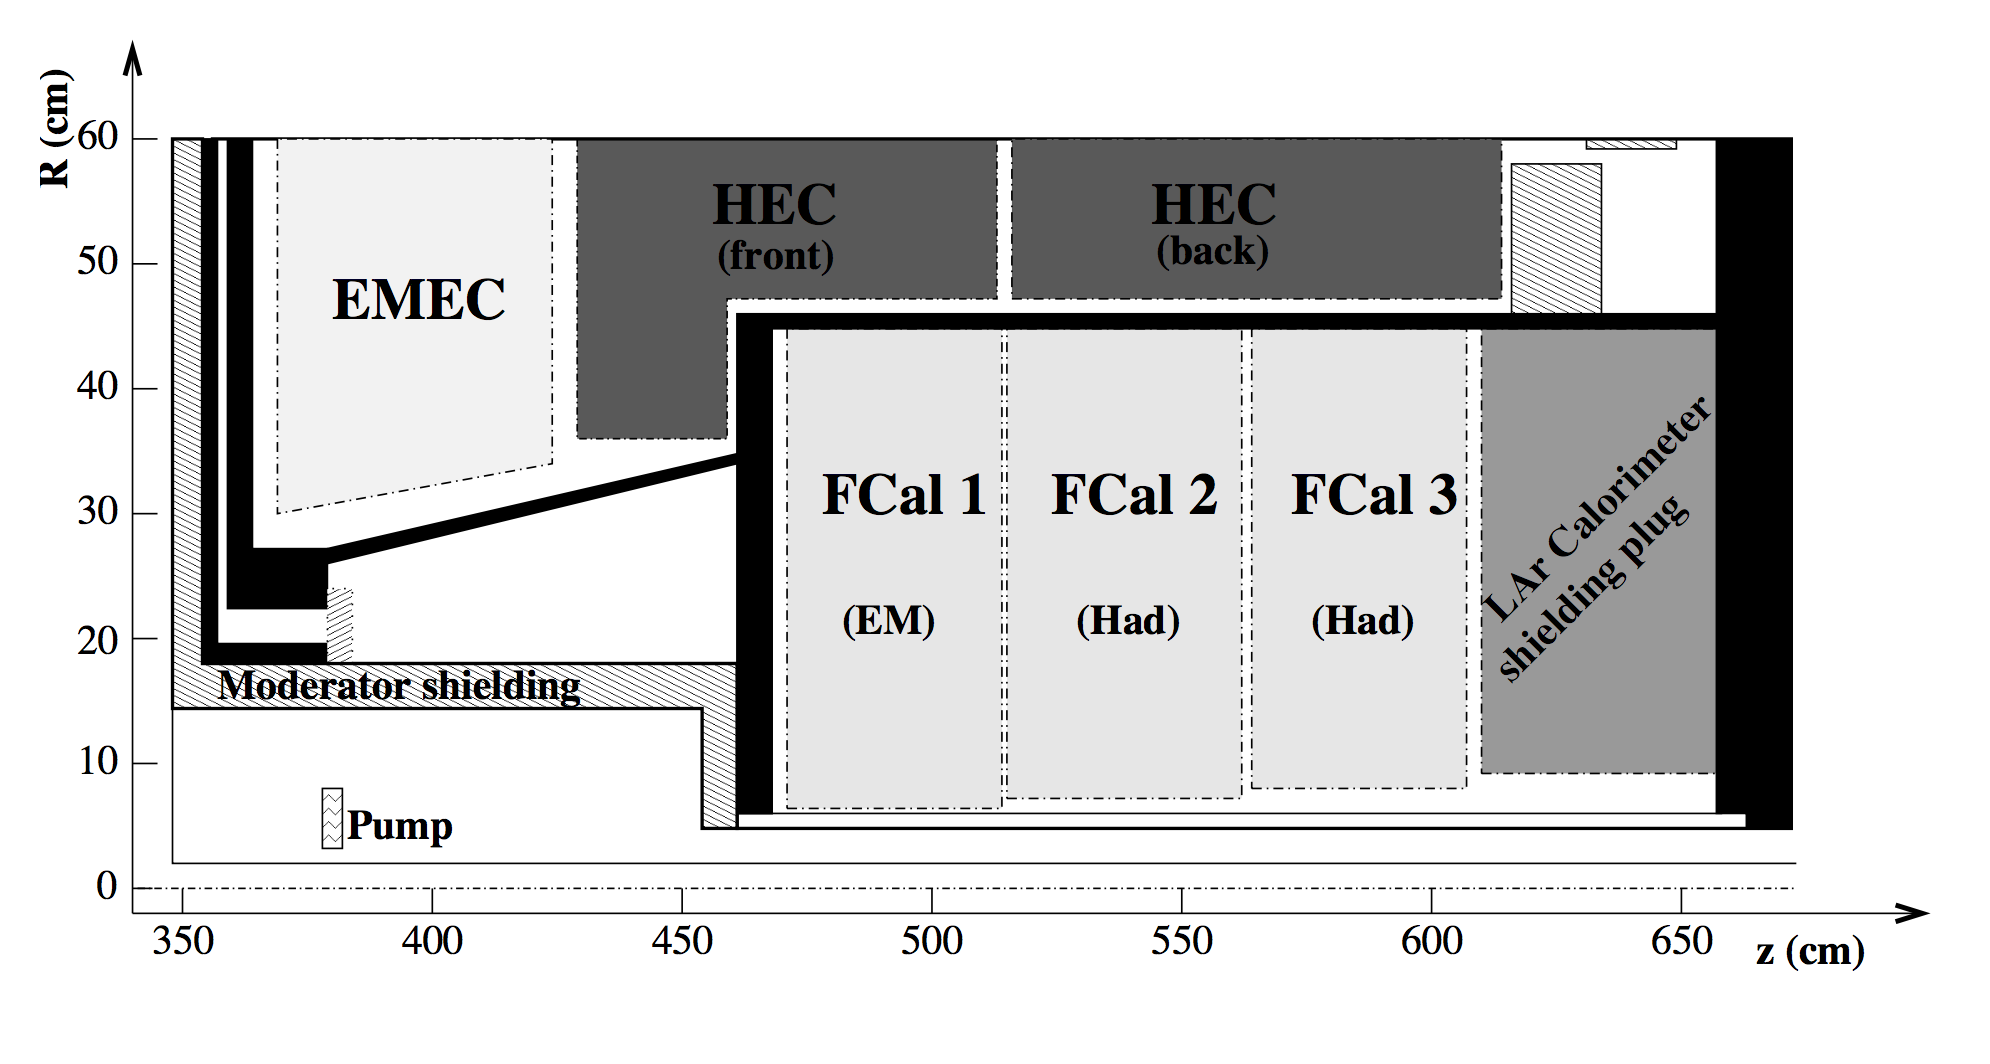
\includegraphics[width=\textwidth]{data/photo/detector/endcap2.png}
\caption{Schematic view for one side of the end-cap and forward calorimeter. One layer of forward calorimeter is electromagnetic and two are hadronic \cite{ATLAS_doc}.}
\label{fig:calorimeter_endcap2}
\end{figure}

\subsubsection{Electromagnetic calorimeter}
In the barrel region, it covers $|\eta| < 1.457$.
In the end-cap region, there are two concentric wheels, with the outer one covering from $1.375 <|\eta| < 2.5$ and the inner one covering from $2.5 <|\eta| < 3.2$.
The EM calorimeter is alternately interleaved with many accordion-shaped layers of electrodes and absorbers, and is filled with liquid argon between the layers at -185$^{\circ}$C .
The accordion geometry provides complete $\phi$ symmetry without azimuthal cracks.
A layer of absorbers is made of a lead plate, to which two stainless-steel sheets (0.2 mm thick) are glued on both sides.
The thickness of the lead plate is 1.53 mm for $|\eta| < 0.8$ and 1.13 mm for $|\eta| > 0.8$ in the barrel region, and 1.7 mm for $|\eta| < 2.5$ and 2.2 mm for $|\eta| > 2.5$ in the end-cap region.
A layer of electrode is made of three conductive copper layers, which are separated by insulating polyimide sheets.
When high energy electrons or photons pass through the lead absorbers, a shower of lower energy electrons, positrons and photons is produced.
The liquid argon atoms, as active material, are ionized by the particles in the shower.
Therefore, free electrons are produced and attracted to the electrode.
By measuring the current from the electrode, the energy of the electron or photon are measured.

The lead absorber can further reduce the energy of particles in the shower before they escape the calorimeter.
Hence, only part of the energy is measured and a correction need to be applied.
The innermost layer, called the presampler, help calculate the correction due to the energy lost.

The EM calorimeter has a fine granularity to have precise energy measurements for electrons and photons.
The granularity depends on the layers, as shown in figure \ref{fig:ECAL}.
Besides the layer of presampler, there are two or three layers (Layer 1, Layer 2 and Layer 3), depending on the $|\eta|$.
In the region of $|\eta|<2.5$, three layers are often used for precise measurements.
Table \ref{tab:granularity_EM_barrel} and \ref{tab:granularity_EM_endcap} show the granularity for each layers in the barrel region and the end-cap region respectively.

\begin{figure}
\centering
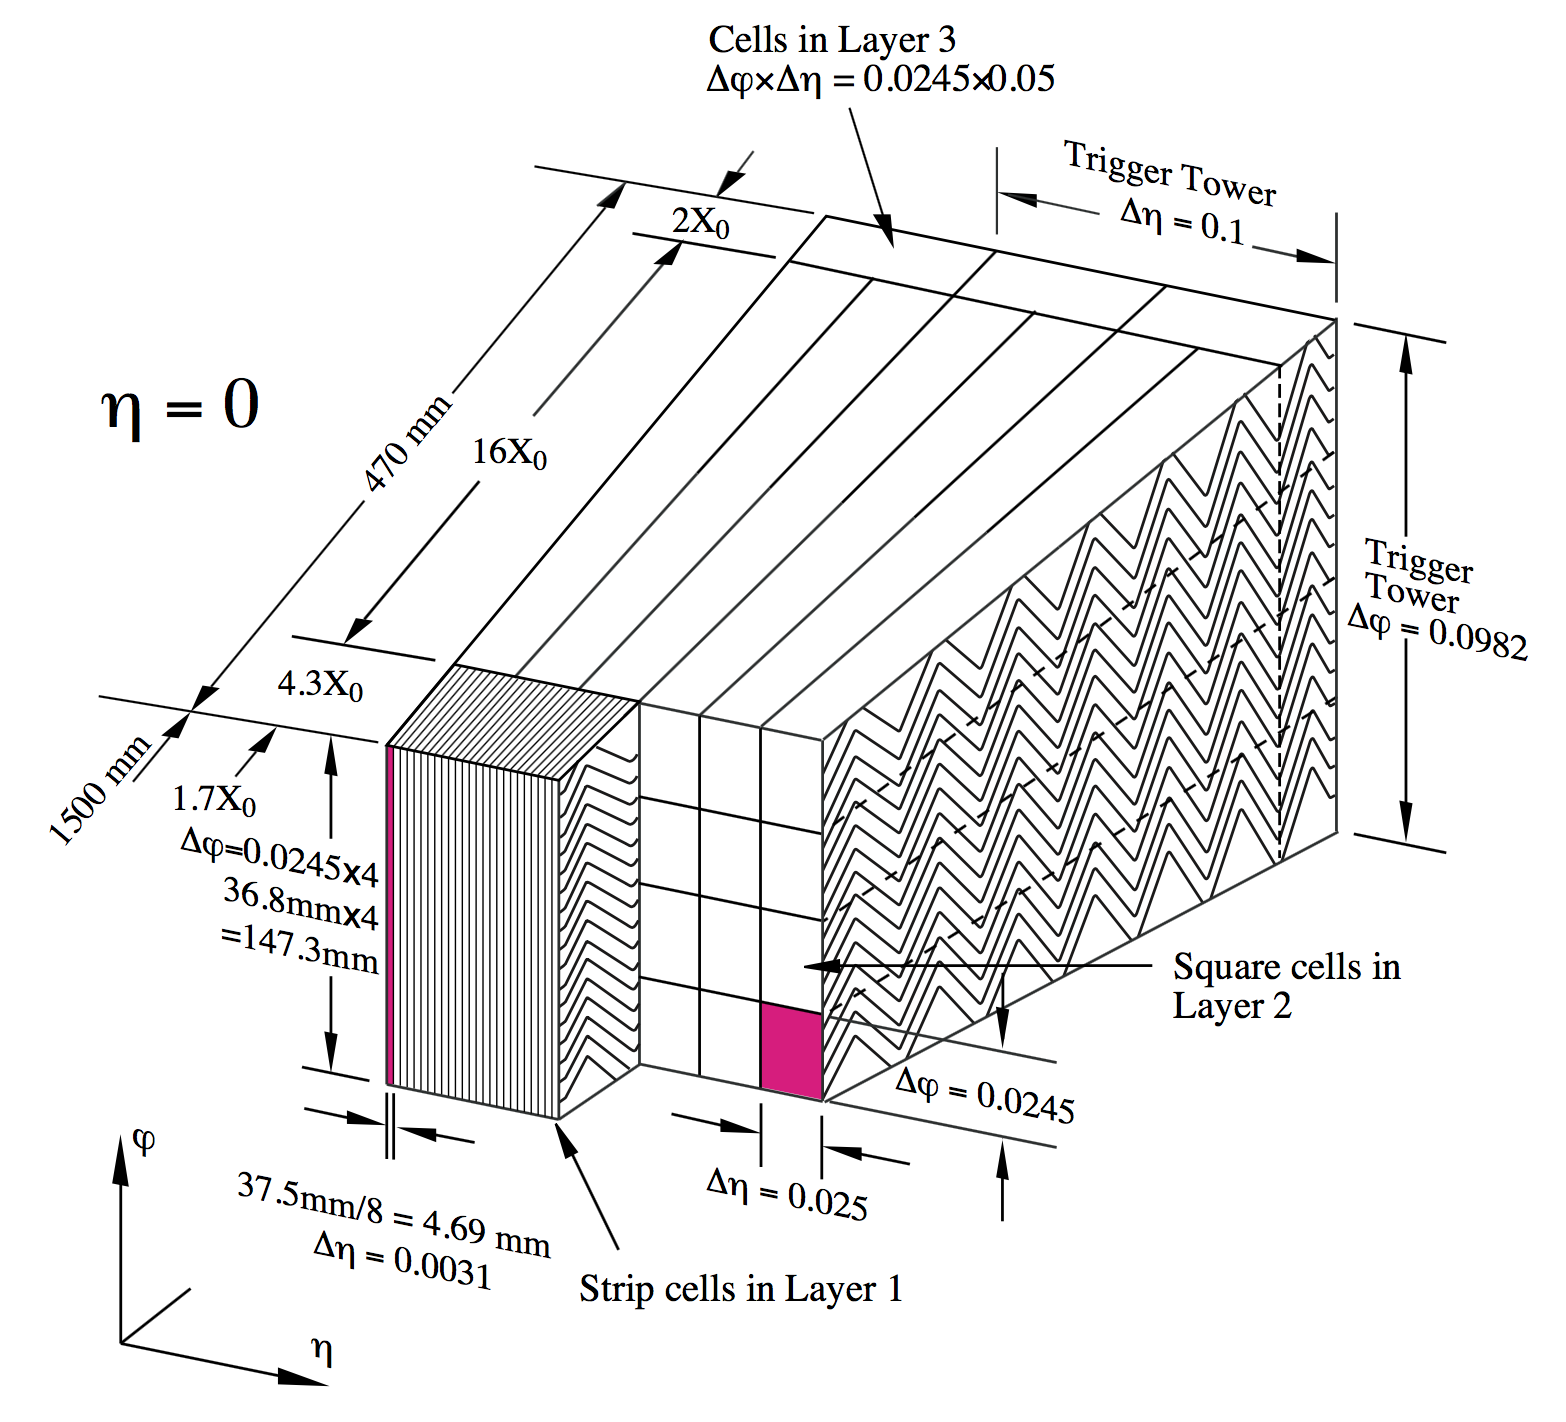
\includegraphics[width=\textwidth]{data/photo/detector/ECAL.png}
\caption{The granularity in $\eta$ and $\phi$ of the cells of each of the three layers in the electromagnetic calorimeter \cite{ATLAS_doc}.}
\label{fig:ECAL}
\end{figure}

\begin{table}[htpb]
\centering
\begin{tabular}{|c|l|r|}
\hline
Layer & $|\eta|$ range & Granularity $\Delta \eta \times \Delta \phi$ \\
\hline
\hline
Presampler & $|\eta| < 1.52$         & $0.025 \times 0.1$ \\
\hline
Layer 1    & $|\eta| < 1.4$          & $0.003 \times 0.1$ \\
           & $1.4 < |\eta| < 1.475$  & $0.025 \times 0.025$ \\
\hline
Layer 2    & $|\eta| < 1.4$          & $0.025 \times 0.025$ \\
           & $1.4 < |\eta| < 1.475$  & $0.075 \times 0.025$ \\
\hline
Layer 3    & $|\eta| < 1.35$         & $0.050 \times 0.025$ \\
\hline
\end{tabular}
\caption{The granularity in $\eta$ and $\phi$ for different layers in the barrel region \cite{ATLAS_doc}.}
\label{tab:granularity_EM_barrel}
\end{table}

\begin{table}[htpb]
\centering
\begin{tabular}{|c|l|r|}
\hline
Layer & $|\eta|$ range & Granularity $\Delta \eta \times \Delta \phi$ \\
\hline
\hline
Presampler & $1.5   < |\eta| < 1.8$   & $0.025 \times 0.1$ \\
\hline
Layer 1    & $1.375 < |\eta| < 1.425$ & $0.050 \times 0.1$ \\
           & $1.425 < |\eta| < 1.5$   & $0.025 \times 0.1$ \\
           & $1.5   < |\eta| < 1.8$   & $0.003 \times 0.1$ \\
           & $1.8   < |\eta| < 2.0$   & $0.004 \times 0.1$ \\
           & $2.0   < |\eta| < 2.4$   & $0.006 \times 0.1$ \\
           & $2.4   < |\eta| < 2.5$   & $0.025 \times 0.1$ \\
           & $2.5   < |\eta| < 3.2$   & $0.1   \times 0.1$ \\
\hline
Layer 2    & $1.375 < |\eta| < 1.425$ & $0.050 \times 0.025$ \\
           & $1.425 < |\eta| < 2.5$   & $0.025 \times 0.025$ \\
           & $2.5   < |\eta| < 3.2$   & $0.1   \times 0.1$ \\
\hline
Layer 3    & $1.5   < |\eta| < 2.5$   & $0.050 \times 0.025$ \\
\hline
\end{tabular}
\caption{The granularity in $\eta$ and $\phi$ for different layers in the end-cap region \cite{ATLAS_doc}.}
\label{tab:granularity_EM_endcap}
\end{table}

\subsubsection{Hadronic calorimeter}
In the barrel region, tile calorimeter is used for measuring the energy of the hadrons in $|\eta| < 1.7$.
The central barrel covers $|\eta| < 1.0$, while the extended region covers $0.8 < |\eta| < 1.7$.
As shown in figure \ref{fig:tile_calorimeter}, the tile calorimeter is alternately interleaved with sheets of steel and scintillator, called tile, like a sandwich.
The steel acts as the absorber material, while the scintillator acts as the active material.
When high energy hadrons pass through the sheets of steel, they strongly interact with the atomic nuclei of the steel, and produce a shower of lower energy charged particles, which then triggers the scintillators to produce photons.
These photons are collected by the wavelength-shifting fibres on the edges of the tile.
The photomultiplier tubes (PMT) then convert the optical signal to an electronic signal.
By measuring the intensity of the photons, the energy of the hadron are measured.
There are 3 layers in the tile calorimeter.
The granularity of the first 2 layers is $\Delta \eta \times \Delta \phi = 0.1 \times 0.1$, while the third layer is $\Delta \eta \times \Delta \phi = 0.2 \times 0.1$.

\begin{figure}
\centering
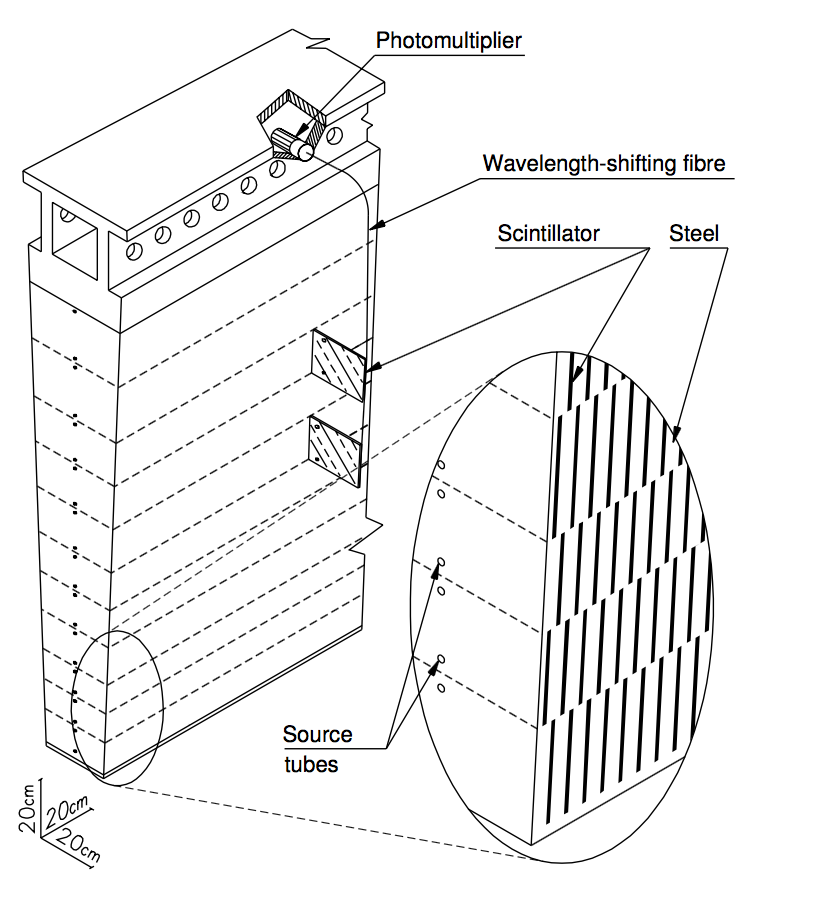
\includegraphics[width=0.7\textwidth]{data/photo/detector/tile.png}
\caption{Schematic view of one module of the tile calorimeter \cite{ATLAS_doc}.}
\label{fig:tile_calorimeter}
\end{figure}

In the end-cap region $1.5 < |\eta| < 3.2$, there are two independent wheels of LAr hadronic calorimeters (HEC) for each end-cap, i.e. the front wheel and the back wheel as shown in figure \ref{fig:calorimeter_endcap2}.
For each wheel, it consists of 32 identical wedge-shaped modules and each module has two layers.
Hence, in total, there are 4 layers for each end-cap.
Similar to the electromagnetic calorimeter, it uses the liquid argon as the active material, but it uses flat parallel copper plates as the absorber material.
On the front wheel, there are 24 copper plates with 25 mm thick.
On the back wheel, there are 16 copper plates with 50 mm thick.
The gap between the copper plates is 8.5 mm.
As shown in figure \ref{fig:HEC}, the gap is separated by three electrodes and is filled with liquid argon.
The granularity is $\Delta \eta \times \Delta \phi = 0.1 \times 0.1$ at $1.5 < |\eta| < 2.5$, and $\Delta \eta \times \Delta \phi = 0.2 \times 0.2$ at $2.5 < |\eta| < 3.2$.

\begin{figure}
\centering
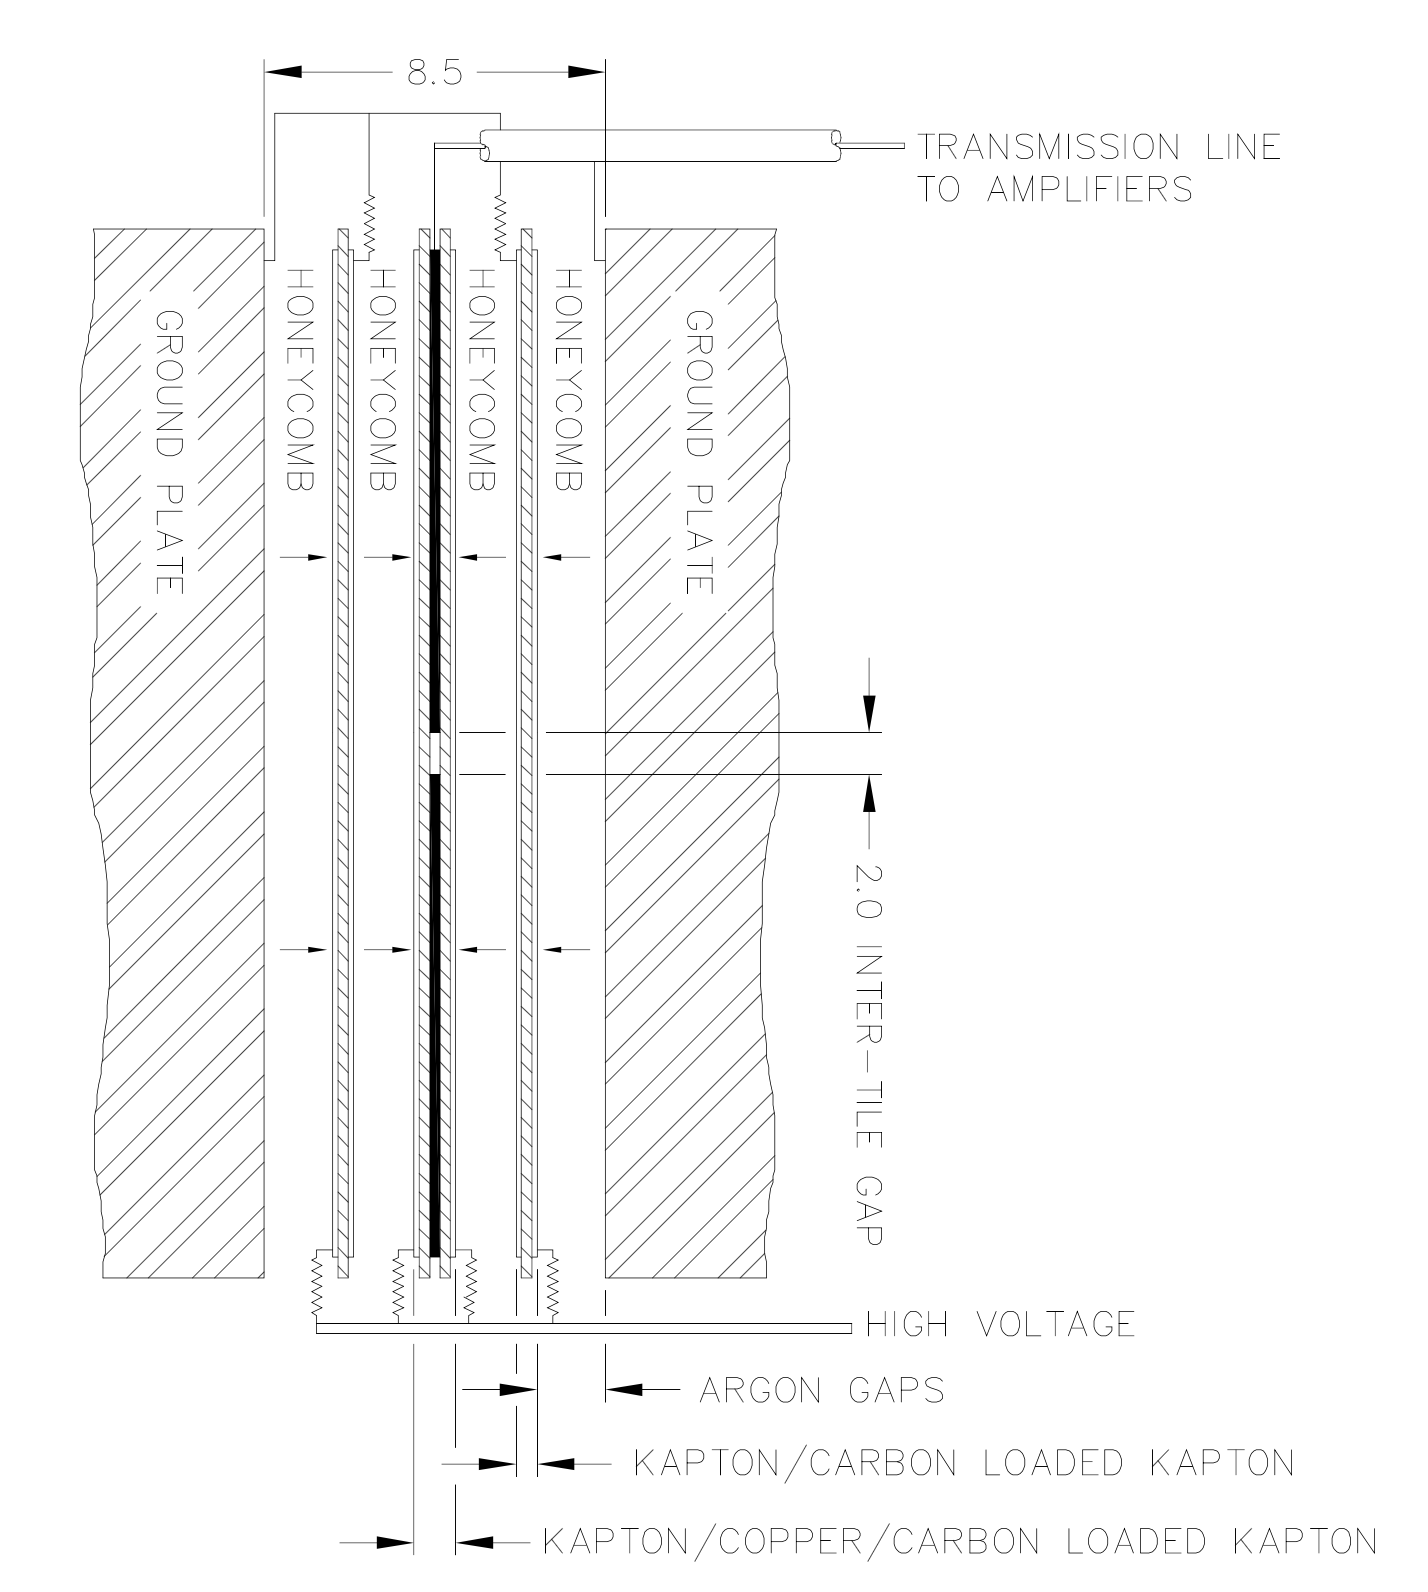
\includegraphics[width=0.7\textwidth]{data/photo/detector/HEC.png}
\caption{Schematic view of the arrangement of the HEC readout structure in the 8.5 mm inter-plate gap. All dimensions are in mm \cite{ATLAS_doc}.}
\label{fig:HEC}
\end{figure}

\subsubsection{Forward calorimeter}
The LAr Forward calorimeter (FCal) covers $3.1<|\eta|<4.9$, with 3 wheels: FCal 1, FCal 2 and FCal 3.
FCal 1 is an electromagnetic calorimeter and uses copper as the absorber material.
FCal 2 and FCal 3 are hadronic calorimeters and use tungsten as the absorber material.
It uses the liquid argon as the active material.

Due to the high $|\eta|$ and the close distance to the interaction point (4.7 m), the forward calorimeters are exposed to high particle fluxes.
This results in a new design with a small gap of liquid argon to avoid the ion build-up problems.
Figure \ref{fig:forward_calorimeter} shows the structure of FCal 1.
A matrix of copper plates is filled inside the forward calorimeter, with 12260 regularly spaced electrodes parallel to the beam direction.
In the electrodes, there are concentric copper rods and copper tubes.
The gap between rod and tube is filled with a thin layer of liquid argon with thickness 0.269 mm.

For FCal 2 and FCal 3, there are 10200 and 8224 electrodes respectively.
The structure is similar to FCal 1, but the copper rods are replaced by the tungsten rods and the matrix of copper plates is replaced by a matrix of tungsten alloy.
The tungsten rod is surrounded by a copper tube with the gap filled with liquid argon.
The thickness of the liquid argon of FCal 2 and FCal 3 are 0.376 mm and 0.508 mm respectively.
The granularity of the forward calorimeter in the x-y plane is shown in \ref{tab:granularity_FCal}.

A shielding plug made of a copper alloy has been mounted behind the FCal 3 to further reduce the backgrounds that reach the muon spectrometer.

\begin{figure}
\centering
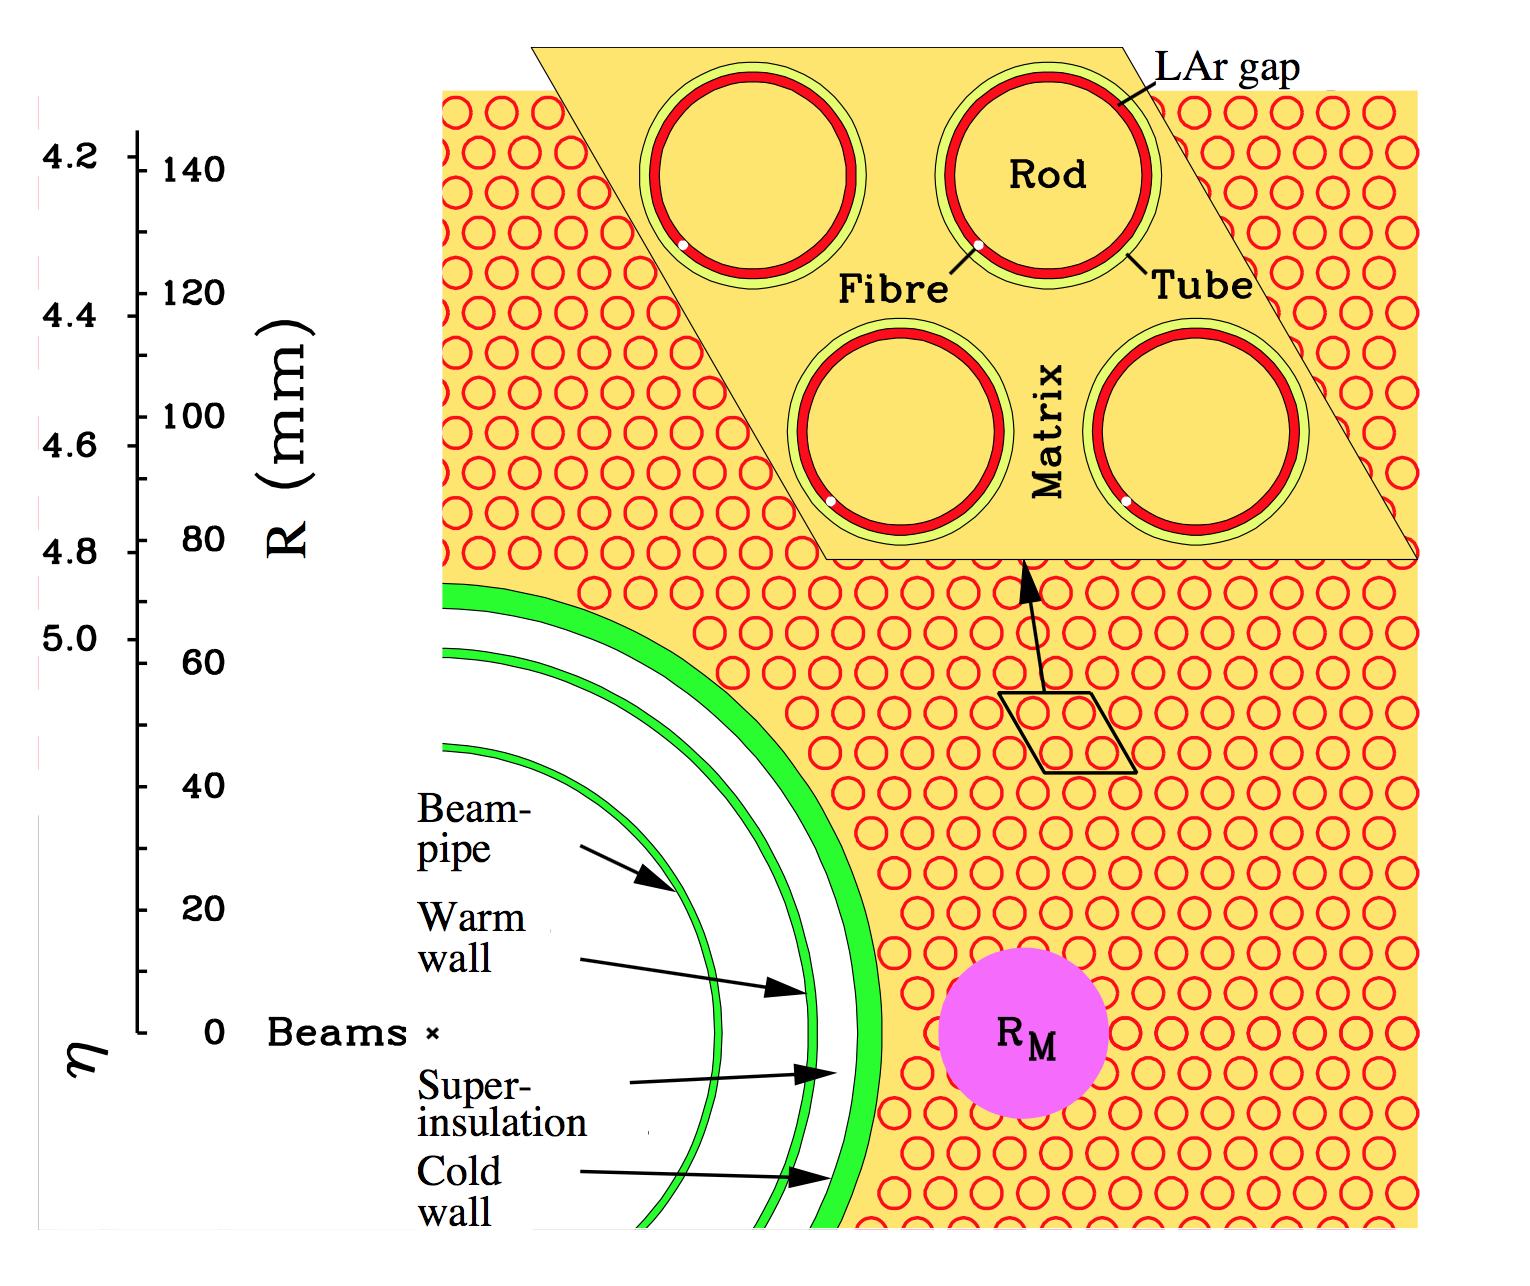
\includegraphics[width=0.7\textwidth]{data/photo/detector/forward.png}
\caption{Electrode structure of FCal 1 with the matrix of copper plates and the copper tubes and rods with the LAr gap for the electrodes. The Moli\`ere radius, $R_M$, is represented by the solid disk \cite{ATLAS_doc}.}
\label{fig:forward_calorimeter}
\end{figure}

\begin{table}[htpb]
\centering
\begin{tabular}{|c|l|r|}
\hline
Layer & $|\eta|$ range & Granularity $\Delta x \times \Delta y$ (cm) \\
\hline
\hline
       & $3.15 < |\eta| < 4.30$   & $3.0 \times 2.6$ \\
FCal 1 & $3.10 < |\eta| < 3.15$   & $\sim$ four times finer \\
       & $4.30 < |\eta| < 4.83$   & $\sim$ four times finer \\
\hline
       & $3.24 < |\eta| < 4.50$   & $3.3 \times 4.2$ \\
FCal 2 & $3.20 < |\eta| < 3.24$   & $\sim$ four times finer \\
       & $4.50 < |\eta| < 4.81$   & $\sim$ four times finer \\
\hline
       & $3.32 < |\eta| < 4.60$   & $5.4 \times 4.7$ \\
FCal 3 & $3.29 < |\eta| < 3.32$   & $\sim$ four times finer \\
       & $4.60 < |\eta| < 4.75$   & $\sim$ four times finer \\
\hline
\end{tabular}
\caption{The granularity in the x-y plane in the forward calorimeter \cite{ATLAS_doc}.}
\label{tab:granularity_FCal}
\end{table}

\subsection{Muon spectrometer}
The muon spectrometer is a tracker for muons.
In the barrel region ($|\eta| < 1.4$), the magnetic field is provided by the barrel toroid, described in section \ref{sec:magnetic_system}.
In the end-cap region ($1.6 < |\eta| < 2.7$), the magnetic field is provided by the end-cap toroid.
In the transition region ($1.4 < |\eta| < 1.6$), the magnetic field is provided by the combined field from the two toroids.

Figure \ref{fig:muon_spectrometer} shows all the components in the muon spectrometer.
The tracking detector is made up of the Monitored Drift Tube chambers (MDT), in the range of $|\eta| < 2.7$.
In the barrel region, the track of a muon is measured by three cylindrical layers of MDT located at R = 5 m, 7.5 m and 10 m, as shown in figure \ref{fig:muon_barrel}.
Each layer has 8 large chambers and 8 small chambers.
In the end-cap and the transition region, there are four wheels of MDT, located at $|z|=$ 7.4 m, 10.8 m, 14 m and 21.5 m, as shown in figure \ref{fig:muon_endcap}.
For the naming scheme of MDT chambers, the first letter (B and E) refers to the barrel and end-cap chambers respectively.
The second letter (I, E, M and O) refers to the inner, extra, middle and outer layers respectively.
The third letter (L and S) refers to the large and small chambers respectively.

\begin{figure}
\centering
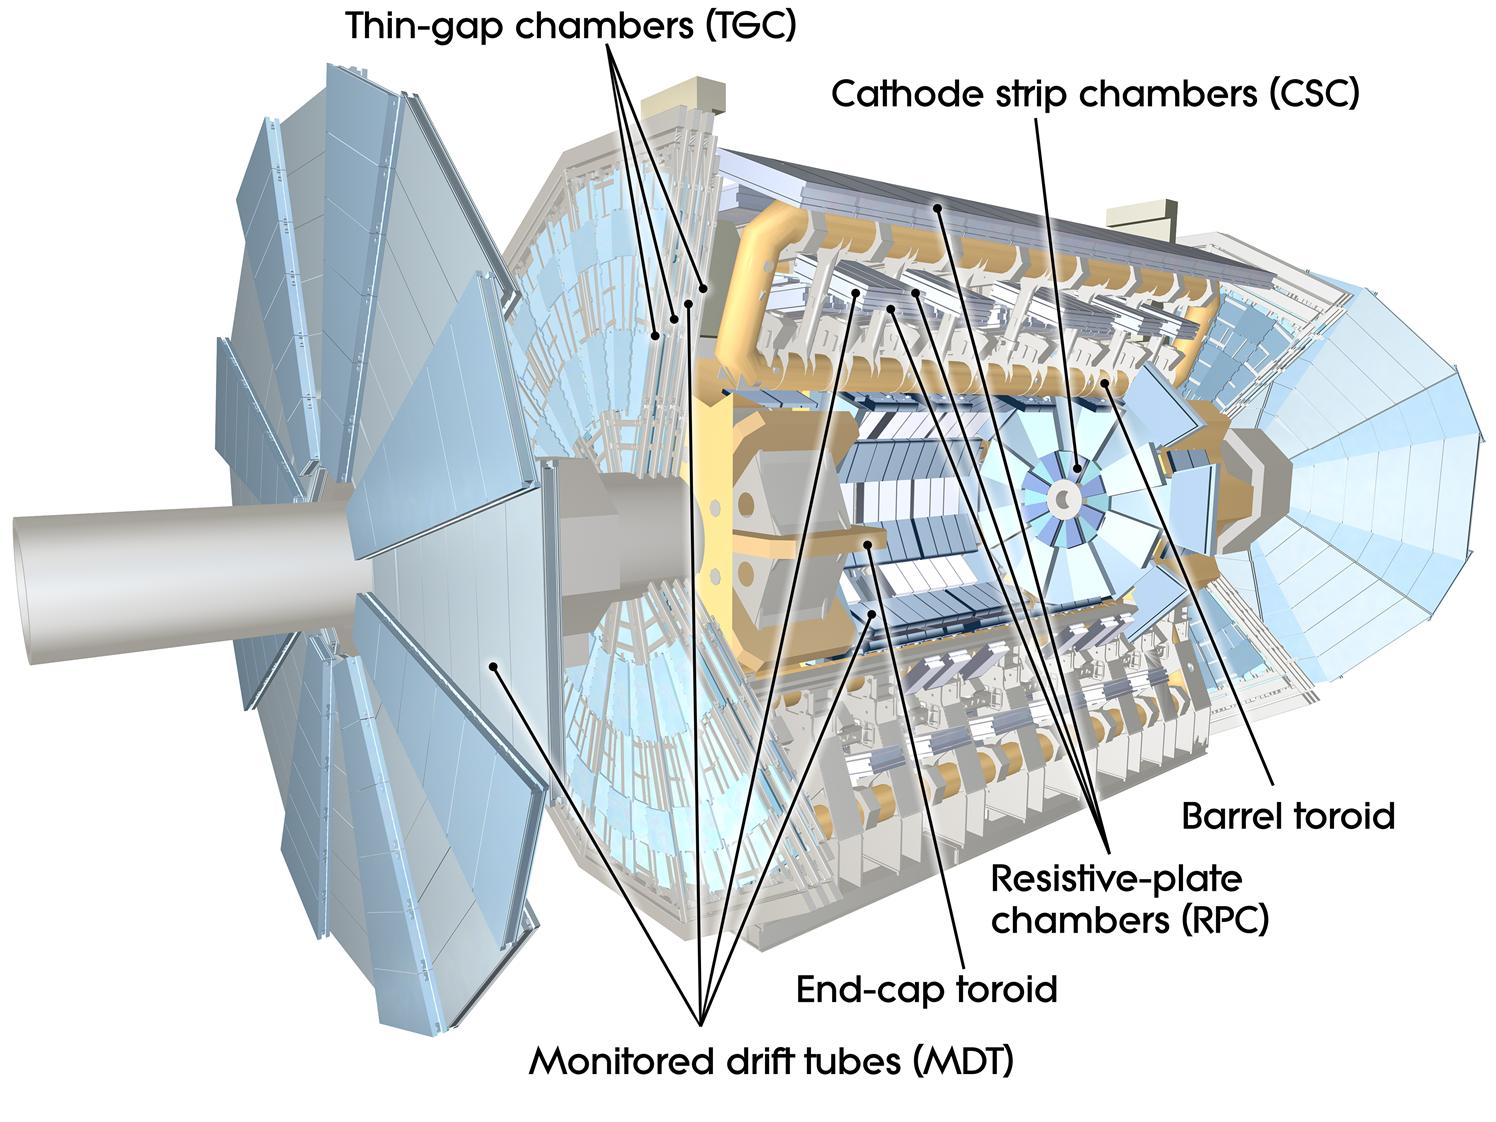
\includegraphics[width=\textwidth]{data/photo/detector/muon_spectrometer.jpg}
\caption{Cut-away view of the muon spectrometer \cite{muon_spectrometer}.}
\label{fig:muon_spectrometer}
\end{figure}

\begin{figure}
\centering
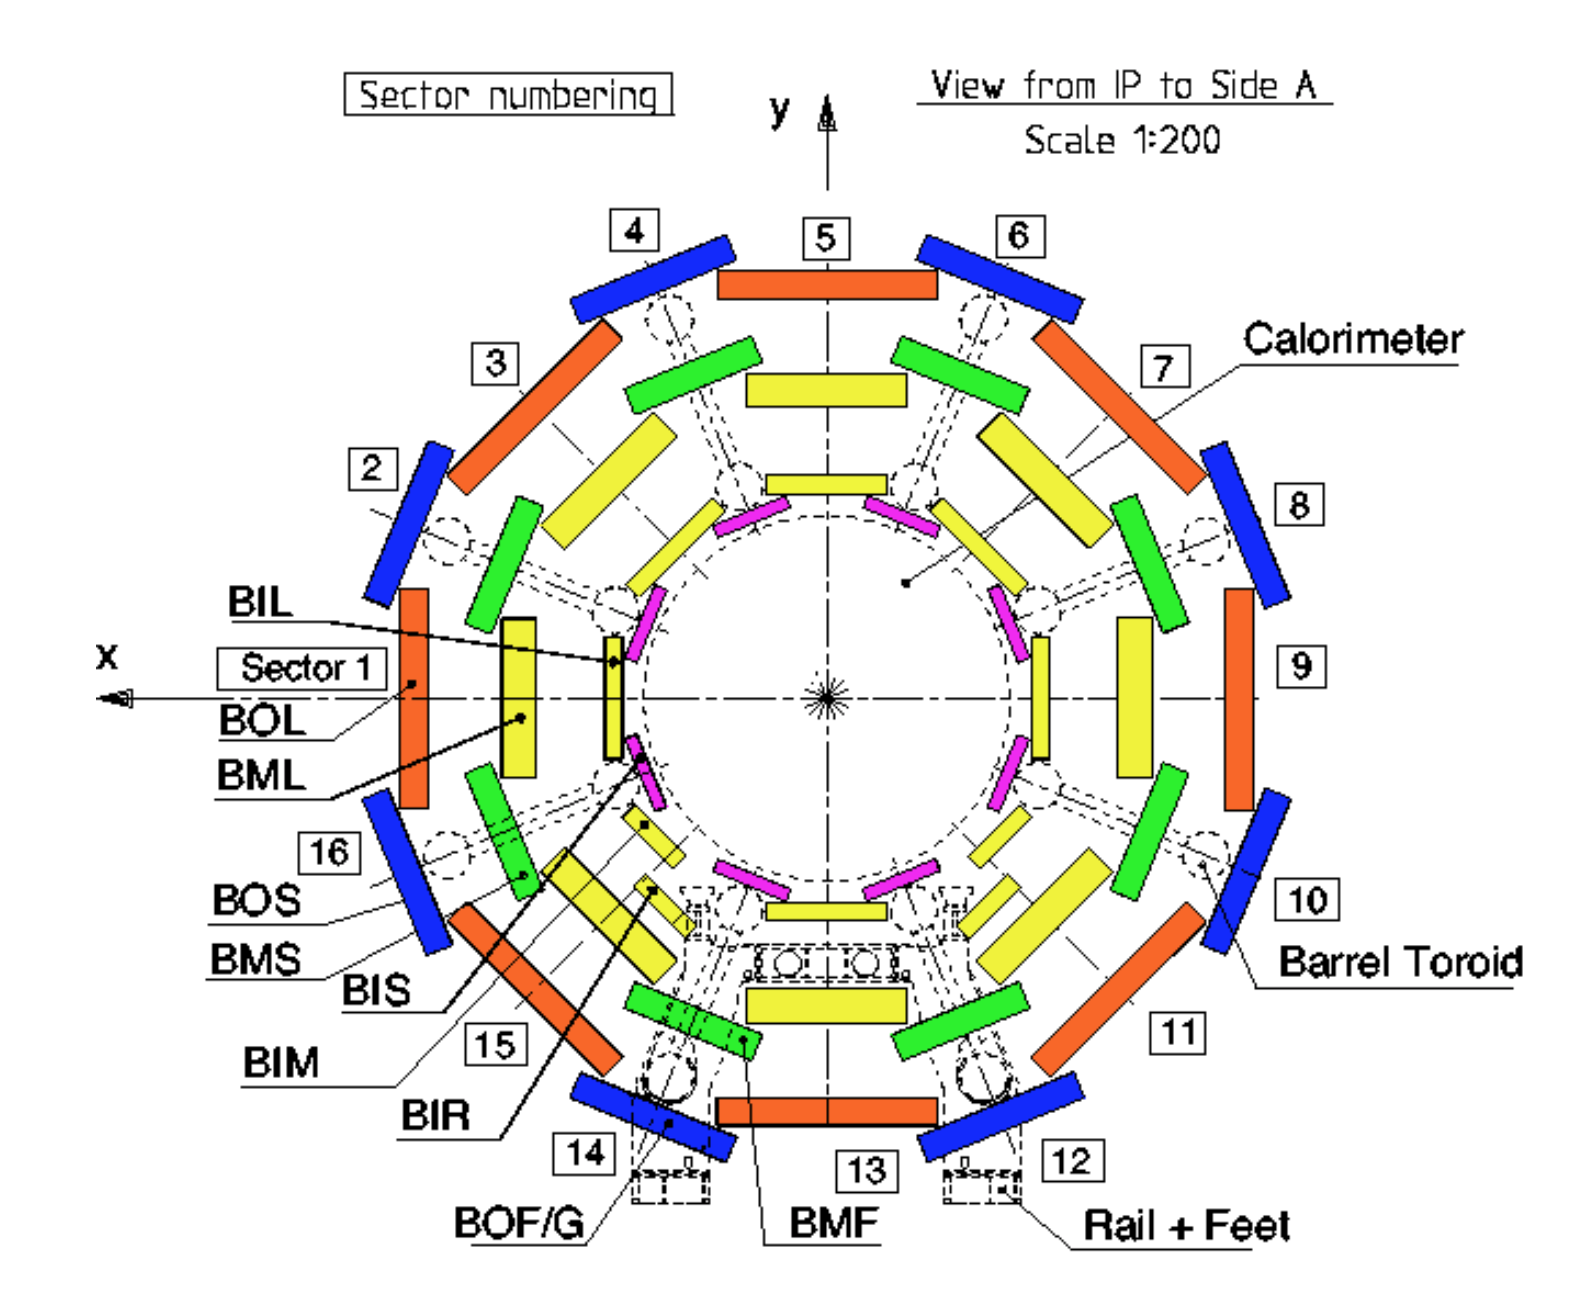
\includegraphics[width=\textwidth]{data/photo/detector/muon_barrel.png}
\caption{The cross section of the barrel region for the muon spectrometer. Three concentric cylindrical layers of barrel MDT are shown \cite{ATLAS_doc}.}
\label{fig:muon_barrel}
\end{figure}

\begin{figure}
\centering
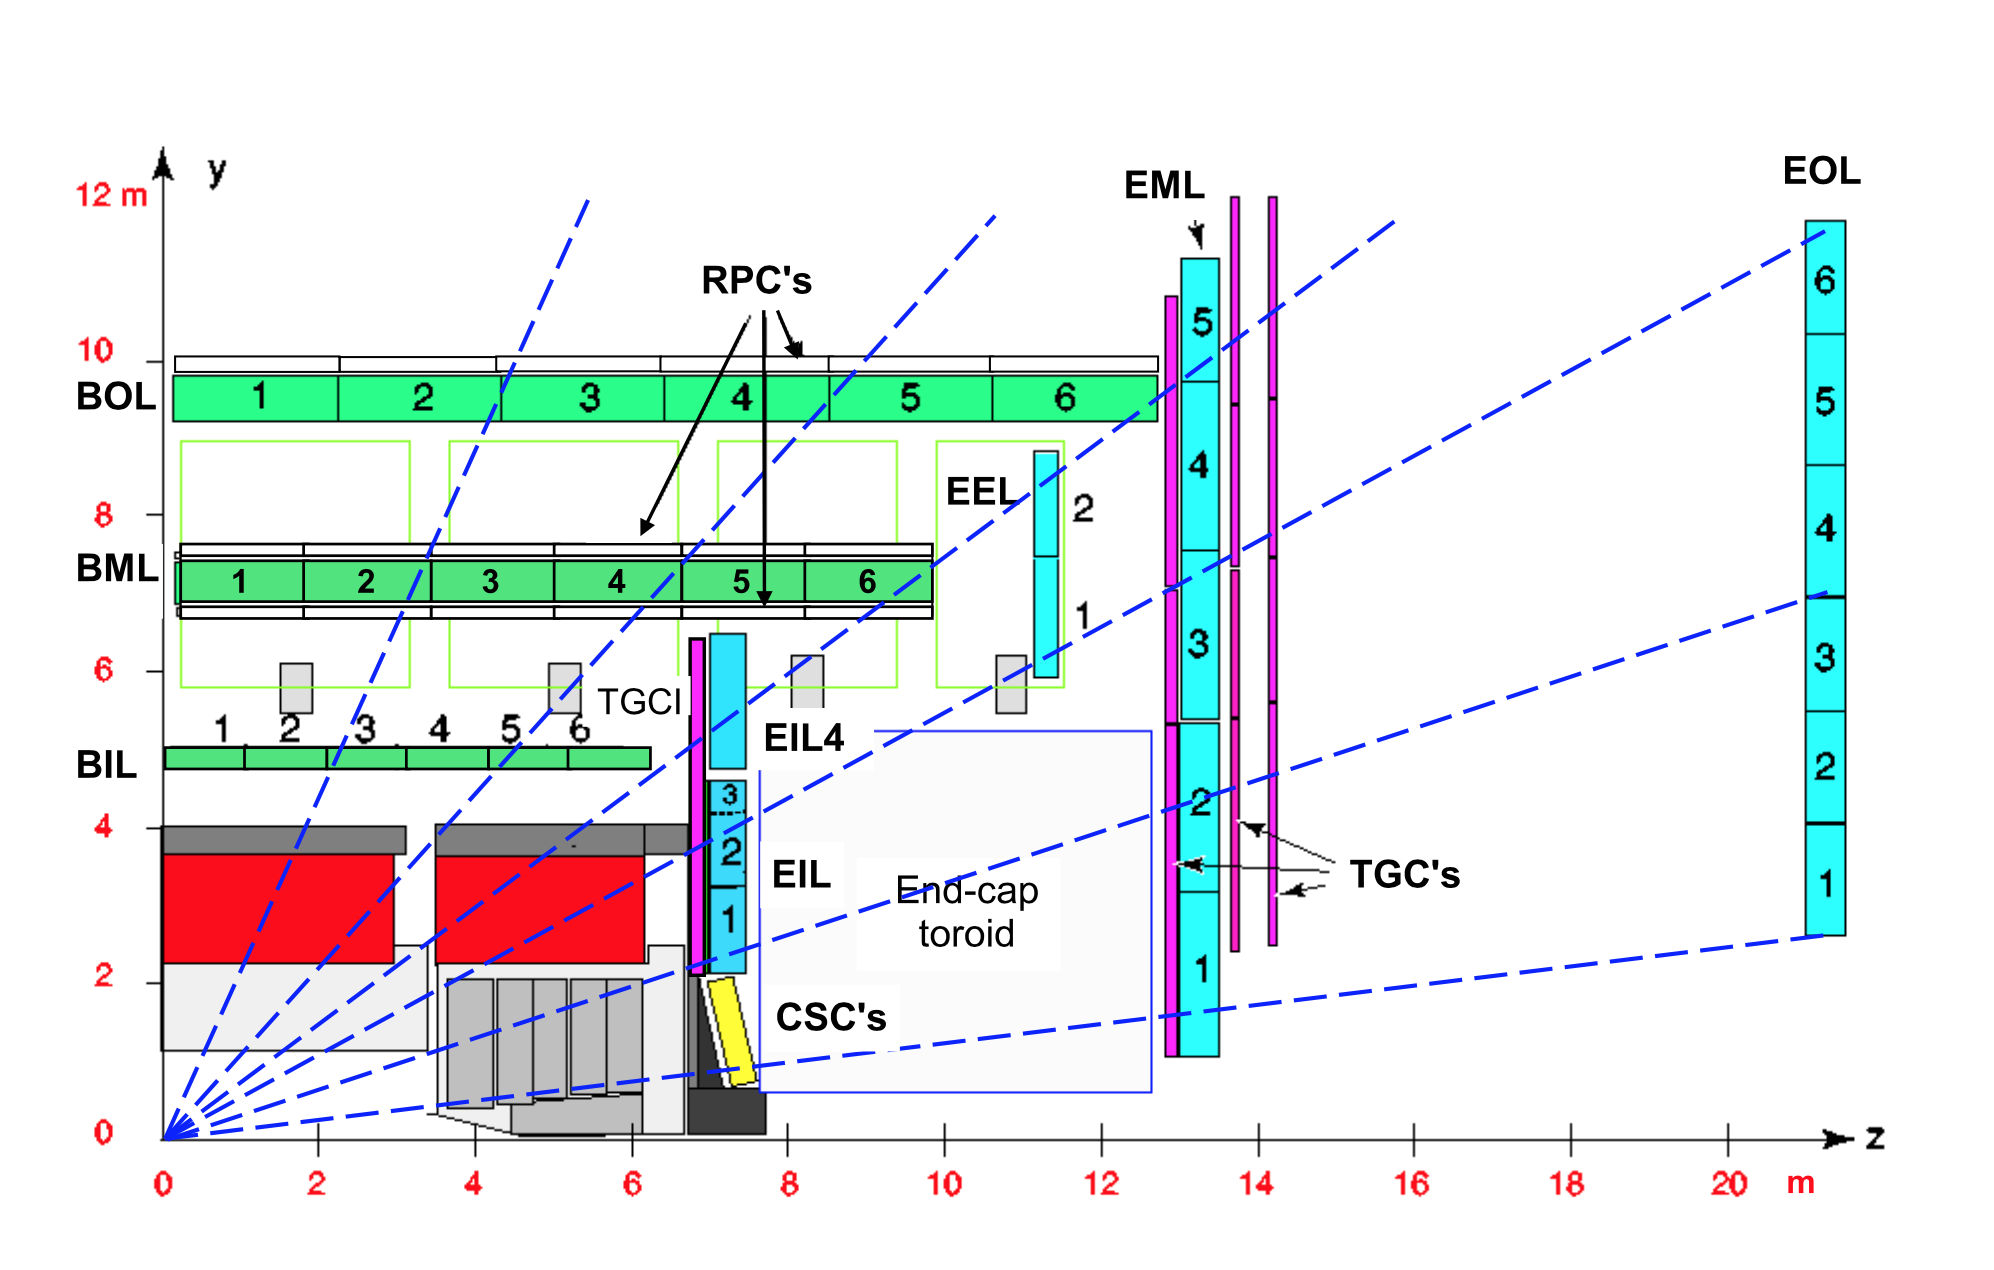
\includegraphics[width=\textwidth]{data/photo/detector/muon_endcap.png}
\caption{The cross section of the end-cap region for the muon spectrometer. Four layers of end-cap MDT are shown in blue colour. Three layers of barrel MDT are also shown in green colour \cite{ATLAS_doc}.}
\label{fig:muon_endcap}
\end{figure}

The total number of drift tubes in each MDT chamber is about 200 to 500 depending on the type of the chamber.
The lengths of the drift tubes vary from 0.85 m to 6.24 m.
The tube is made of aluminium with a diameter of 29.970 mm as shown in figure \ref{fig:MDT}.
It is filled with a gas mixture of 93\% argon and 7\% CO$_2$, operated at a pressure of 3 bar.
The anode wire is made of tungsten-rhenium with a diameter of 50 $\mu$m, at an electric potential of 3080 V.
When muons pass through the tube, the gas is ionized and free electrons are produced, which are attracted and drift to the anode wire.
By measuring the drift time the free electrons take from the position of the muon to the anode wire, the position of the muon can be measured.
The average resolution of the MDT is 80 $\mu$m per tube, or about 35 $\mu$m per chamber.

\begin{figure}
\centering
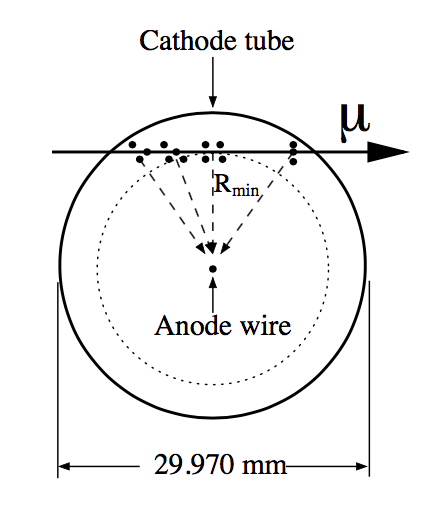
\includegraphics[width=0.5\textwidth]{data/photo/detector/MDT.png}
\caption{The cross-section of a MDT tube. When muons pass through the tube, free electrons are produced along the track, which drift to the anode wire \cite{ATLAS_doc}.}
\label{fig:MDT}
\end{figure}
